%                                                                 aa.dem
% AA vers. 7.0, LaTeX class for Astronomy & Astrophysics
% demonstration file
%                                                 (c) Springer-Verlag HD
%                                                revised by EDP Sciences
%-----------------------------------------------------------------------
%
%\documentclass[referee]{aa} % for a referee version
%\documentclass[onecolumn]{aa} % for a paper on 1 column  
%\documentclass[longauth]{aa} % for the long lists of affiliations 
%\documentclass[rnote]{aa} % for the research notes
%\documentclass[letter]{aa} % for the letters 
%
\documentclass[structabstract]{aa}  
%\documentclass[traditabstract]{aa} % for the abstract without structuration 
                                   % (traditional abstract) 
%
\usepackage{graphicx}
%%%%%%%%%%%%%%%%%%%%%%%%%%%%%%%%%%%%%%%%
\usepackage{txfonts}
%%%%%%%%%%%%%%%%%%%%%%%%%%%%%%%%%%%%%%%%
%
%\usepackage{xtab}
\usepackage{epsfig}
\usepackage{natbib}
\usepackage{lscape}
\usepackage{wasysym}
\usepackage{array}
\usepackage{amssymb}
\usepackage{subfigure}
%\usepackage{multicol}
\usepackage{longtable}
%\usepackage{supertabular}
\usepackage{rotating}
\usepackage{color}
\usepackage{colortbl}
\usepackage{soul}
\usepackage[normalem]{ulem}
\usepackage{fancyheadings}
\bibpunct{(}{)}{;}{a}{}{,}

\newcommand\T{\rule{0pt}{2.6ex}}
\newcommand\B{\rule[-1.2ex]{0pt}{0pt}}

\begin{document}
%
   \title{Metallicity of M dwarfs}

   \subtitle{III. Planet-metallicity and planet-stellar mass correlations of the HARPS GTO M dwarf sample \thanks{Based on observations made with the HARPS instrument on the ESO 3.6-m telescope at La Silla Observatory under programme ID 072.C-0488(E)
   }}

\author{ V. Neves\inst{1,2,3} \and X. Bonfils\inst{2} \and
  N. C. Santos\inst{1,3} \and X. Delfosse\inst{2} \and
  T. Forveille\inst{2}  \and F. Allard\inst{4}  \and
  S. Udry\inst{5}}

\institute{
Centro de Astrof{\'\i}sica, Universidade do Porto, Rua das Estrelas,
4150-762 Porto, Portugal \\
email: {\tt vasco.neves@astro.ua.pt}
\and
UJF-Grenoble 1 / CNRS-INSU, Institut de Plan\' etologie et
d'Astrophysique de Grenoble (IPAG) UMR 5274, Grenoble, F-38041,
France.
\and
Departamento de F\'{\i}sica e Astronomia, 
Faculdade de Ci\^{e}ncias, Universidade do Porto, 
Rua do Campo Alegre, 4169-007 Porto, Portugal
\and
Centre de Recherche Astrophysique de Lyon, UMR 5574: CNRS,
Universit\'e de Lyon, \'Ecole Normale Sup\'erieure de Lyon, 46 All\'ee
d'Italie, F-69364 Lyon Cedex 07, France
\and
Observatoire de Gen\`eve, Universit\'e de Gen\`eve, 51 Chemin des
Maillettes, 1290 Sauverny, Switzerland
}

   \date{Received XXX; accepted XXX}

% \abstract{}{}{}{}{} 
% 5 {} token are mandatory
 
  \abstract
  % context heading (optional)
  % {} leave it empty if necessary  
   {}
  % aims heading (mandatory)
   { The aim of this work is the study of the planet-metallicity and the planet-stellar mass correlations of the HARPS GTO M dwarf subsample.}
  % methods heading (mandatory)
   { We use a new method that takes advantage of the HARPS high-resolution spectra to increase the precision of metallicity. We reach a precision of 0.08 dex for [Fe/H].}
  % results heading (mandatory)
   {The well-known correlation for giant planets with metallicity is present. Regarding Neptunians and smaller hosts no correlation is found and there is even a hint that an anti-correlation might exist. We only have eight planet hosts in our sample. Therefore, more detections are needed to confirm or deny these results. Regarding stellar mass, a possible correlation with planets was discovered, but was found to be the result of a detection bias.}
  % conclusions heading (optional), leave it empty if necessary 
   {}

\keywords{stars: fundamental parameters -- 
stars: late type --
stars: atmospheres --
stars: planetary systems
}


   \maketitle
%
%________________________________________________________________

\section{Introduction}
\label{intro}
%\textcolor{red}{Still don't know if I'm going to write a full introduction or just a resume of the previous paper and 3/4 paragraphs.}

\textbf{Mass and metallicity are two important observables directly connected to the formation and evolution of planetary systems. These quantities play an important role in} core-accretion models of formation and evolution of planets around M dwarfs and other stars, as shown by numerous works studying the relationship of both quantities with planet formation \citep[e.g.][]{Ida-2005,Kornet-2006, Kennedy-2008a, Thommes-2008, Alibert-2011, Mordasini-2012}. 

%The planets that orbit M dwarfs form in a different environment than solar-type and higher mass stars, as 

The initial conditions of planet formation (disk mass, temperature and density profiles, gravity, gas-dissipation and migration timescales...etc.) all change with stellar mass \citep[e.g.][]{Ida-2005, Kornet-2006, Kennedy-2008a, Alibert-2011}.  \textbf{Metallicity also plays a major role in the efficiency of the formation of giant planets for FGK dwarfs, as shown by both models \citep[e.g.][]{Ida-2004b} and observational data, \textbf{in the form of a metallicity-planet correlation} \citep[e.g.][]{Gonzalez-1997,Santos-2004b,Fischer-2005, Sousa-2011b, Mayor-2011}, but seems to vanish for Neptunian and smaller planet hosts \citep[]{Sousa-2008,Bouchy-2009, Ghezzi-2010,Sousa-2011b}.}



Recently, it has been shown that the planet-metallicity correlation may also be true for M dwarfs \citep[e.g.][]{Bonfils-2007,Johnson-2009, Schlaufman-2010, Rojas-Ayala-2012, Terrien-2012}. \textbf{However, more detections of planets around M dwarfs and a more precise metallicity determination are needed to achieve higher confidence levels that remain low, around the $\sim$2~$\sigma$ level \citep{Bonfils-2007,Schlaufman-2010}. In this context it is important to use a volume-limited sample of stars, as several planet-hunting programs targeting FGK dwarfs have metallicity-biased samples \citep[e.g.][]{Baranne-1996,Fischer-2005b,Melo-2007} }.


According to \citet{Thommes-2008} and \citet{Mordasini-2012}, a lower metallicity can be compensated by a higher disk mass to allow giant planet formation (and vice-versa -- the so called `compensation effect'). This result implies that M dwarfs can form giant planets, but only if they have high metallicities, thus suggesting \textbf{an even stronger} planet-metallicity correlation compared to FGK dwarfs. 


%Moreover, the metallicity effect may be independent or only slightly dependent on the stellar mass effect \citep{Johnson-2010,Alibert-2011}. \textbf{Furthermore, it remains to be seen} if the planet-metallicity correlation that seems to vanish for Neptunian and smaller planet hosts around FGK dwarfs \citep[]{Sousa-2008,Bouchy-2009, Ghezzi-2010,Sousa-2011b} and predicted by models \citep[e.g.][]{Mordasini-2012} is observed for M dwarfs \citep[e.g.][]{Rojas-Ayala-2012,Terrien-2012}. \textcolor{red}{remove this paragraph? - put the references in another section.}



%Ida 2005 and Kornet 2006 consider that giant formation around more massive stars than the sun is less likely, in contrast with KK2008a

% Kornet 2006 concludes that jupiter hosts are more common around less massive stars, that differs from Laughlin 2004 and Ida 2005.

% Mordassini 2009 a,b --> using only solar mass, b is more important. About PMC (feh).

% Mardasini 2012 --> feh effect is confirmed for giant planets. no feh effect for neptunians and for SE it might be an anti-correlation. No correlation between feh and distance for giant planets. low feh planets start further out, but migrate more, while at high feh they start closer in but migrate less! disk masses and giant planets are correlated. disk lifetime acts as a threshhold for giants formation. There is a compensation effect between mass and feh. feh effect is stronger when disk mass is weaker and vice versa.

% Laughlin 2004 - formation of giants around M dwarfs is inhibited.

%Ida 2004 - Gas giants and range of metallicities --> dependence of gas giant formation on feh

%Ida 2005 - lower mass planets may be more common around M dwarfs, because M dwarfs tend to migrate before starting gas accretion. The formation of Giant planets around M dwarfs is inhibited.

% Ida 2008b, Ida 2010 - frequency of SE around solar type stars

% discuss the question about disk lifetimes?

% Alibert 2010 --> study on mass with planet formation efficiency. The minimum metallicity required to form a massive planet is correspondingly lower for massive stars than lower mass stars.





Disk instability models \citep[e.g.][]{Boss-1997}, on the other hand, do not predict\textbf{, in general,} the dependence of the planet formation \textbf{on} stellar mass \citep[e.g.][]{Boss-2006a} and metallicity \citep{Boss-2002}. %\textcolor{red}{Should we detail the feh dependent models? All of them Mayer(2007), Cai 2007, etc -- see Sarah Seager's book. fail to fragment. (!)}
%\textbf {or predict a slight dependence on [Fe/H] \citep[e.g.][]{} -TBD }. 
Contrary to the core-accretion paradigm \citep{Pollack-1996}, the formation of planets does not originate from the collisional accretion of planetesimals, but from the collapse of an unstable part of the protoplanetary disk, forming in a timescale of thousands of years when compared to a timescale of Myrs for core-accretion models. Observational evidence, however, has shown that there is a dependence between planet occurrence and both stellar mass and metallicity \citep[e.g.][]{Santos-2004b,Bonfils-2007, Lovis-2007, Johnson-2007, Johnson-2010, Sousa-2011b, Mayor-2011} \textbf{over a wide range of dwarf types (AFGKM)}, thus favoring the core-accretion scenario as the primary mechanism of planet formation, at least for closer-in planets. 

In this context, the pollution scenario \citep[e.g.][]{Murray-2002,Gonzalez-1997}, defends that the observed enhanced metallicity is only at the surface of the photosphere, and that the formation of planets occurs at all metallicities, thus supporting disk instability models. Observationally, this would translate, for M dwarfs into a non-detection of the planet-metallicity correlation, as M dwarfs have very deep convective layers and are expected to be fully convective at masses below 0.4 M$_{\odot}$. However, as we have seen, most studies hint or demonstrate the presence of the metallicity correlation for giant planets, thus signaling a primordial origin of the presence of metals.

%\textbf{For the case of hot Jupiters around FGK stars, the occurrence rate} is no bigger than 2\% \citep[e.g.][]{Howard-2010,Mayor-2011,Wright-2012}. On M dwarfs this number may be even lower, as shown by both works on models \citep[e.g.][]{Laughlin-2004,Ida-2005, Kennedy-2008a} and observations \citep[e.g.][]{Endl-2006, Cumming-2008,Johnson-2010,Bonfils-2011}. \textbf{In fact, there is only one hot jupiter detection orbiting an M-type star so far \citep{Johnson-2012}\textcolor{red}{confirm this...}}. The paucity of hot jupiters around M dwarfs is most probably due to an inefficient planet-formation process around M dwarf protoplanetery disks (Laughlin-2004, Ida-2005, Kennedy-2008a). Whether or not this paucity of close-in Gas giants around M dwarfs extends to higher periods and beyond the snow line remains to be seen. \textcolor{red}{NOTE: Wright 2012 is about FGK not M. Is Johnson 2012 the only detection so far?}

%\citet{Gould-2010} estimates\textbf{, from microlensing events between 2005 and 2008}, that the frequency of giant planets beyond the snow line around low mass stars can be as high as $36\pm15\%$. However, the upper limits and frequencies for different period regions from 1 to 10.000 days calculated by \citet{Bonfils-2011} taking into account the detection limits of radial velocity of M dwarfs shows that the frequency of \textbf{1-10 M$_{J}$ planets, for a period between 1.000 and 10.000 days,} is only $4^{+5}_{-1} \%$, and it is even lower for shorter periods. \textbf{This result is compatible with the frequency of 3.6\% for M stars obtained by \citet{Johnson-2010}.}  \textcolor{red}{This last part is open for discussion, of course.}. Previous works \citep{Butler-2006,Johnson-2007,Cumming-2008} publish an even lower planet fraction for M dwarfs ($\sim$ 2\%) for periods below 2000 days.}


\textbf{In the course of this paper we implement a new method to derive the metallicities of \textbf{a volume-limited} sample of 102 M dwarfs from the HARPS GTO programme. This method uses the high-resolution spectra of HARPS to achieve a [Fe/H] precision of 0.08 dex and is described in the Appendix. Then,} we
%to refine and enhance the precision of metallicities based on the photometric calibration of \citet{Neves-2012}, itself a refinement of the work of\citet{Schlaufman-2010}. Then, we use this determinations, as well as stellar mass determinations calculated using the mass-luminosity relation of \citet{Delfosse-2000} 
search for correlations between the frequency of planets with stellar mass and metallicity. In Sect. \ref{sample}, we describe our M dwarf sample and observations using the HARPS spectrograph. Then, in Sect. \ref{relation}, we investigate the stellar mass/metallicity correlations with the frequency of planets. Afterwards, we calculate the detection limits of the sample, to check for biases, and to test the stellar mass-planet relation.
%the planet detections accumulate in the higher end of stellar mass and lower end of V magnitude. 
Finally, we discuss our results in Sect. \ref{discussion}.




%The fact that ho 



%Efficiency of giant planets should increase with stellar mass (Laughlin 2004, Ida 2005b Kennedy 2007)

%No clear metallicity effect is found in the Neptunian mass domain and at lower masses even an anti-correlation might exist. (Mordassini 2012)

%Disk gas masses and giant planet masses are correlated (Mordassini 2012). 

%BUT Microlensing surveys show that 

%Mdisk is proportional to the Mdisk^alphad



%Alibert 2011 states that the number of embryos that eventually evolve and form planets are a growing function of the stellar mass. 

%The minimum metallicity required to form a massive planet is correspondingly lower for massive stars than lower mass stars. 
%
%However, \citet{Alibert-2011} states that the metallicity efffect is only weakly dependent on stellar mass. 

%--> Talk about the paucity of jovians around M dwarfs

%--> Should we talk about Disk instability?









%__________________________________________________________________

\section{Sample and Observations}
\label{sample}

Our 102 M dwarf sample is described in detail in Sect. 2 of \citet{Bonfils-2011}. It is a volume limited (11 pc) sample, containing stars with a declination $\delta< +20^{\circ}$, with V magnitudes brighter than 14  mag and including only stars with a projected rotational velocity $vsini\le 6.5$ km/s. All known spectroscopic binaries and visual pairs with separation lower than 5 $arcsec$, as well as previously unknown fast rotators were removed \textit{a priori} or \textit{a posteriori} from the original sample. All stars were surveyed for planets with the HARPS spectrograph \citep{Mayor-2003b}.


From the 102 M dwarf stars, a total of 14 planets are currently detected, in 8 systems, from which 3 have more than one planet.\textbf{ Table \ref{planets} shows the planet hosts, planets, and planetary mass and Period taken from \citet{Bonfils-2011}, except in the case of Gl 433c and Gl 876e, taken from \citet{Delfosse-2012} and \citet{Rivera-2010} respectively.. We refer to Table 1 of this paper for the full planet parameters and respective references. Table \ref{full_table} depicts the sample used in this paper, where columns 2 and 3 list the right ascension and declination respectively, column 4 the parallaxes and their respective uncertainties, column 5 the source of the parallax, column 6 the spectral type of the M dwarf, and columns 7 and 8 the V- and K$_{s}$-band magnitudes respectively. Finally, columns 9 and 10 contain the calculated stellar mass and metallicity.}

%\textcolor{red}{should we put here the Table 1 of Bonfils(2011) but only including our sample? Should we put more information regarding the sample(observations? YES TBD.}

\begin{table}[h]
\centering
\caption{Planet host stars in the sample, along with the planetary mass and Period. We refer to \citet{Bonfils-2011} for the full references.}
\label{planets}
\begin{center}
%\resizebox{9cm}{!}{
\begin{tabular}{l l r r r }

\hline
\hline
star & planet & \multicolumn{2}{c}{$m\sin{i}^{\dag}$} & Period \\
     &        &  [M$_{\oplus}$] & [M$_{j}$]     & [days] \\
\hline
Gl 176 & b &  8.4 & 0.026 &  8.7(8) \\
Gl 433 & b &  6.4 & 0.0202 &  7.36(5) \\
Gl 433$^{1}$ & c & 44.6 & 0.14 & 3(693) \\
Gl 581 & b & 15.7 & 0.0492 &  5.368(7)\\
Gl 581 & c &  5.4 & 0.017 & 12.9(3) \\
Gl 581 & d &  7.1 & 0.022 & 66.(8) \\
Gl 581 & e &  1.9 & 0.0060 &  3.1(5) \\
Gl 667C & b &  6.0 & 0.019 &  7.20(3) \\
Gl 667C & c &  3.9 & 0.012 & 28.1(5) \\
Gl 674 & b & 11 & 0.034 &  4.6(9) \\
Gl 832 & b & 200 & 0.64 & 3(416) \\
Gl 849 & b & 310 & 0.99 & 18(52) \\
Gl 876 & b & 839 & 2.64 & 61.0(7) \\
Gl 876 & c & 264 & 0.83 & 30.2(6) \\
Gl 876 & d &  6.3 & 0.020 &  1.9378(5) \\
Gl 876$^{2}$ & e & 14.6 & 0.046 & 124.(26) \\
\hline
\hline
\end{tabular}
%}
\end{center}
\raggedright
$\dag$ The true mass (m$_{p}$) is reported for Gl876b,c \citep{Correia-2010}. \\
$^{1}$ \citet{Delfosse-2012}\\
$^{2}$ \citet{Rivera-2010} 
\end{table}




The stellar masses were calculated using the empirical mass-luminosity relationship of \citet{Delfosse-2000}, using stellar parallaxes, taken mostly from the HIPPARCOS catalogue \citep{van_Leeuwen-2007} , but also from \citet{van_Altena-1995, Jahreiss-1997, Hawley-1997, Henry-2006}. The V band magnitudes were taken from the Sinbad database\footnote{http://simbad.u-strasbg.fr/simbad/}), and the infrared K$_{s}$ magnitudes from 2MASS \citep{Skrutskie-2006}. The stellar mass values range from 0.09 to 0.60 $M_{\odot}$, with a mean and median values of 0.32 and 0.29 $M_{\odot}$ respectively. We note that, Gl 803, a young ($\sim 20$ Myr) M dwarf star in our sample, with a circumstellar disk \citep{Kalas-2004}, has a derived stellar mass value of 0.75, too high for a M dwarf. Therefore, the stellar mass calibration being used may not be adequate \textbf{for the youngest} M dwarfs. 

The metallicities were first calculated with the photometric calibration provided by \citet{Neves-2012}, using stellar parallaxes, and V and K$_{s}$ magnitudes. 
%\textcolor{red}{Neves or Schlaufman calibration? It's very hard to choose one, but the Schlaufman has a higher rms = 0.11, although it also has a wider range of metallicities. BUT we can compare it with the metallicity of 451GTO, and here the Schlaufman one clearly wins.}. 
\textbf{To improve on precedent photometric calibrations, we try to root the metallicity effect in the high-resolution HARPS spectra,} using the measurements of the equivalent widths of the lines and features of the 26 red orders (533-691 nm region) of the HARPS spectra. \textbf{The new calibration is detailed in the Appendix}. We achieve an increase in precision with the new calibration reaching a [Fe/H] dispersion of the order of 0.08 dex. The metallicity values range from -0.88 to 0.32 dex, with a mean and median values of -0.13 and -0.11 dex respectively. We note that there is a slight offset towards lower metallicities when compared with the 582 FGK dwarfs from the HARPS-2 volume-limited sample \citep{Sousa-2011b} with mean and median values of -0.10 and -0.08 dex respectively, but it is statistically negligible.
%\textbf{The metallicity difference to the volume-limited and kinematically-matched sample of \citet{Schlaufman-2010}, from the Geneva Copenhagen survey \citep[GCS -- ][]{Nordstrom-2004,Holmberg-2007,Holmberg-2009}  , with a mean of -0.14 dex is, however, negligible}.

%\textcolor{red}{Note: Using the calibration of SL10 as a starting point for the feh spectroscopic calibration we have a mean of -0.12 and a median of -0.10 dex. Is the use of the spectra pushing the metallicities towards lower values, due to the molecular lines?? NO! The photometric calibrations of SL10 and Neves-2012 have even worse results (mean = -0.18, median = -0.14) BUT the SL10 puts the mean metallicity at -0.17! And the SN from GCS is -0.15.. But the end the differences are small, because the uncertainties are significative.}.

%\textcolor{red}{A table with masses and metallicities for the first 10 stars is needed in here, I think. DO for all stars and put in the end, TBD}

The observations were gathered using the HARPS instrument \citep{Mayor-2003b,Pepe-2004}, installed at the ESO 3.6-m telescope at the La Silla observatory in Chile. It is a high resolution (R$\sim$115000) spectrograph in the visible, covering a region between 380 and 690 nm. During the time of the GTO program, from 11th February 2003 to the 1st of April 2009, a total of 1965 spectra were recorded. The aim of the HARPS M dwarf programme is to achieve a $\sim 1$ m/s RV precision per exposure for the brightest targets. The chosen recording mode during this period was single fiber mode, that relies only on a single calibration but gives enough precision to reach the aim of the programme. Using single fiber mode has the advantage of obtaining non-contaminated spectra that can be used to perform other studies \textbf{other that measuring the star's RV, such as measuring activity diagnostics, using Ca II H and K lines,} and calculating stellar parameters and abundances. A more detailed description of the observations is given in Sect. 3 of \citet{Bonfils-2011}.

\section{Stellar mass, metallicity, and planets}
\label{relation}

In this section we use the new metallicity values (see the Appendix) as well as the stellar mass determinations to study the possible correlations of these quantities with the planet frequency. 

%\textbf{We recall that in the M dwarf sample paper \citep{Bonfils-2011}, all planets are detected in the most massive half (resp. brightest half) of the stellar mass (resp. V-mag) distribution. This means that a stellar mass distribution may be subject to detection biases: one the one hand the reflex motion induced by the planetary companions is higher in lower mass stars, meaning a higher RV signal but on the other hand, the higher mass stars are brighter,meaning a higher signal-to-noise ratio, and thus a better RV precision. Here, we want to investigate if this trend is due to an observational bias or if it is physical in nature.}



%as shown in \citet{Bonfils-2011} paper, that 

%\textbf{We recall that in the M dwarf sample paper \citep{Bonfils-2011}, all planets are detected in the most massive half (resp. brightest half) of the stellar mass (resp. V-mag) distribution. } 

\textbf{Fig. \ref{histmass} shows the histogram of the stellar mass distribution of the whole sample. The solid blue and dashed vertical lines represent the mean and the median of the stellar mass of the sample respectively. The black vertical lines locate the systems with planet detections. }

\textbf{We can see that the planet detections are all on one side of the median of our sample distribution with stellar mass (all detected planets are around the more massive stars), as previously shown by \cite{Bonfils-2011}. This is also true for the V magnitude distribution (all detected planets are around the brighter stars). Therefore, any result described in this section regarding stellar mass will be checked in Sect. \ref{dl}, because its distribution may be subject to detection biases: on the one hand the reflex motion induced by the planetary companions is higher in lower mass stars, meaning a higher radial velocity (RV) signal, but on the other hand, the higher mass stars are brighter, meaning a higher signal-to-noise ratio, and thus a better RV precision.}

\textbf{A lower star count in the ]0.35-0.40] M$_{\odot}$ bin of Fig. \ref{histmass} is observed. To check whether this feature is real or due to a small number statistical fluctuation we did a simple monte-carlo simulation by generating 100.000 virtual samples containing 102 stars in the ]0.05-0.65]  M$_{\odot}$  region, using an uniform distribution generator. Then, for each sample, we searched for a bin, in the ]0.15-0.5] region, where the count difference with both adjacent bins was the same or higher than in the observed stellar mass distribution. To this end we chose a count difference of 6,7, and 8, obtaining a frequency of 10.6, 5.1, and 2.2\% respectively. We thus attribute the low number of stars with a mass between 0.35 and 0.4 M$_{\odot}$ to a small number statistical fluctuation.} 

\textbf{It is assumed that metallicity is not influenced by detection biases, due to the fact that we are using a volume-limited sample.} 

\textcolor{red}{(I wonder why Fig 4. and Fig 1. of Bonfils 2011 are a bit different..... :O)}

\begin{figure}[h]
\begin{center}
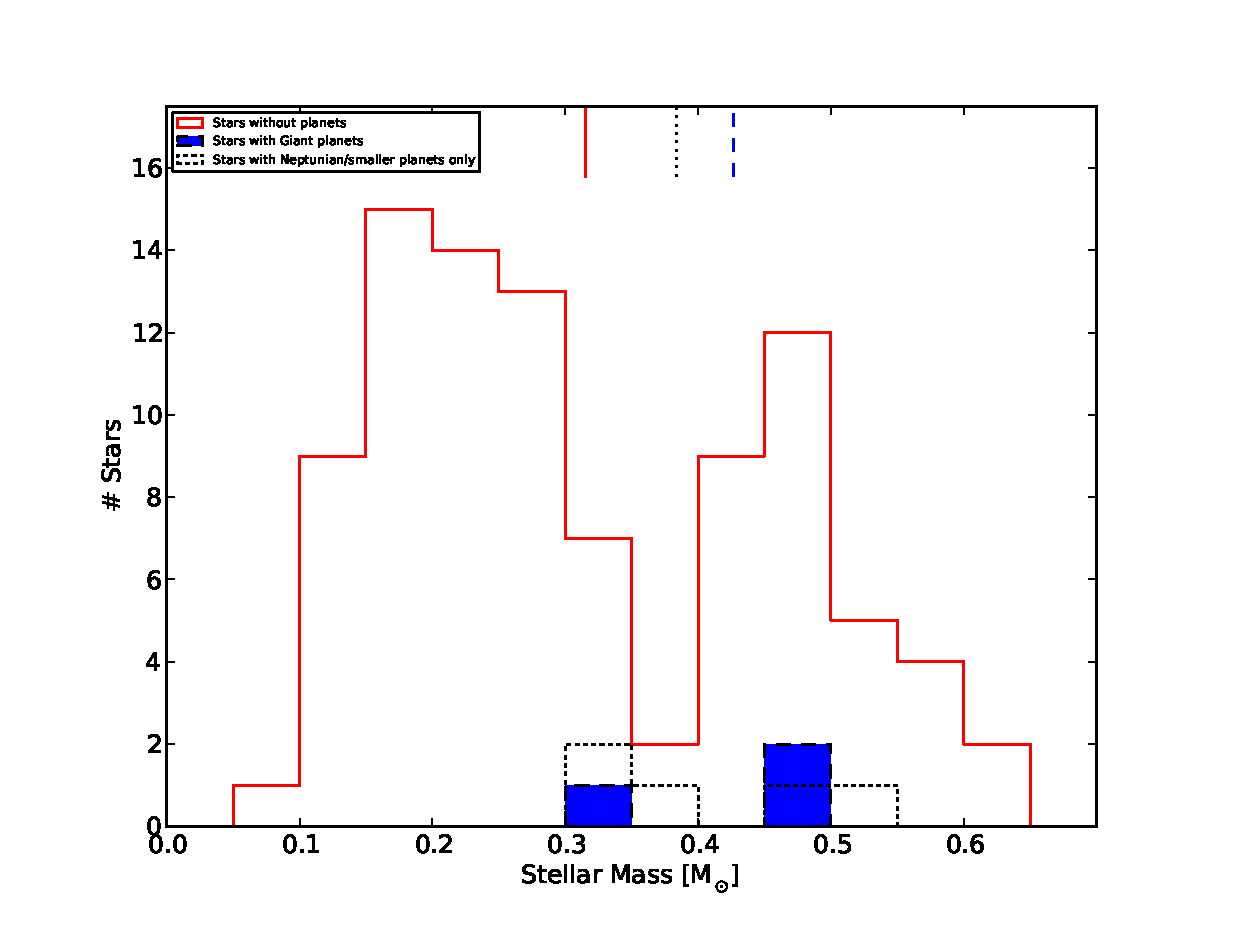
\includegraphics[scale=0.45]{../harpsm/all/pics_harpsmgtovpaper/histmass.eps}
\end{center}
\caption{Stellar mass distribution of the sample. The blue solid and dashed vertical lines represent the mean and the median of the stellar mass of the sample respectively. The black vertical lines locate the systems with planet detections.}
\label{histmass}
\end{figure}

%as planets are easier to detect around more massive stars. In fact, the Fig. 1 of \citet{Bonfils-2011} (and Fig. \ref{histmass} of this work) shows that 

Figure \ref{histfull} shows the histograms of metallicity (upper panel) and stellar mass (lower panel) of our sample. The solid red histograms represent the stars without planets, while the filled dashed blue histograms the stars with Jovians planets, and the dotted black histograms the star with Neptunians/smaller planets only . The vertical solid red, dashed blue, and dotted black lines above each histogram depict the value of the mean of each distribution. 

%We note that there is a lower count in the 0.35-0.40 M$_{\odot}$ bin. We attribute this to statistical fluctuations due to the small number of each bin. \textcolor{red}{what else???}.


\begin{figure}[h]
\begin{center}
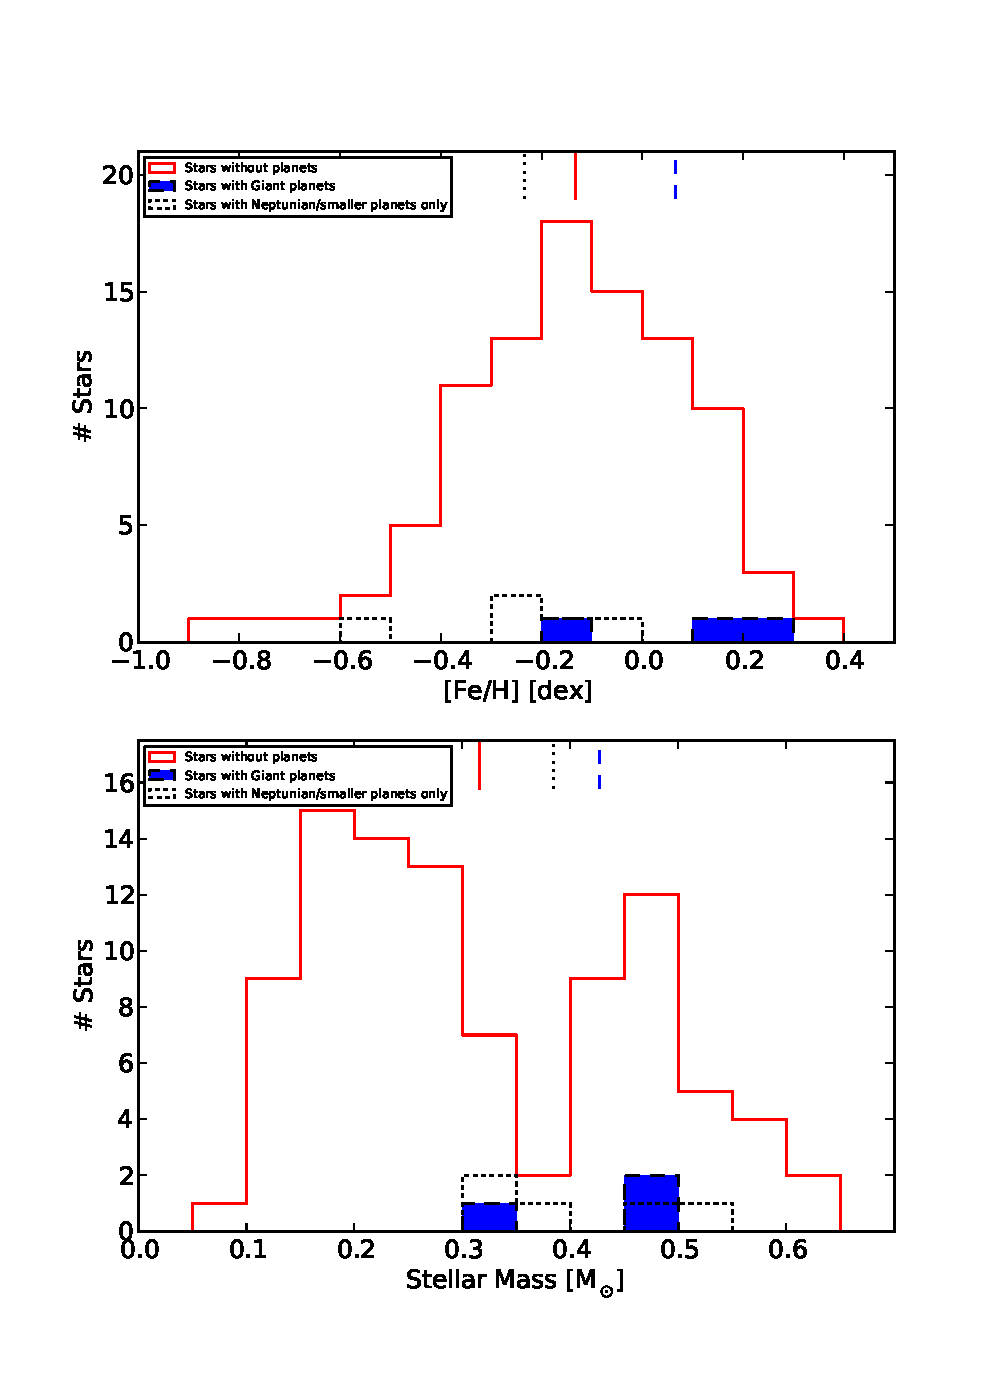
\includegraphics[scale=0.6]{../harpsm/all/pics_harpsmgtovpaper/histfull.eps}
\end{center}
\caption{Histograms of stars without planets (solid red), with Jovian planets (filled dashed blue), and with Neptunians/smaller planets (dotted black) for stellar mass (upper panel) and metallicity (lower panel). The vertical solid red, dashed blue, and dotted lines above the histograms represent the mean of each distribution, respectively.}
\label{histfull}
\end{figure}


\textbf{We can observe in Table \ref{planets} that, for metallicity, the difference of the averages (medians resp.) of the full sample between planet and non-planet host distributions is small (0.01 and -0.07 dex, respectively). For stellar mass, there is a 0.09 $M_{\odot}$ (0.13 $M_{\odot}$ resp.) difference between the averages (medians resp.) of planet and non-planet host histograms.} 

\begin{table}[h]
\centering
\caption{Difference of averages and medians between planet host and non-planet host distributions.}
\label{planets}
\begin{center}
\resizebox{9cm}{!}{
\begin{tabular}{l r r }

\hline
\hline
[Fe/H] & Diff. of averages & Diff. of medians \\
 & [dex] & [dex] \\
%\hline
Full sample (N$_{h}$=8) & 0.01 & -0.07 \\
Jovians hosts (N$_{h}$=3) & 0.20 & 0.26 \\
Neptunian/smaller hosts (N$_{h}$=5) & -0.10 & -0.10 \\
\hline
Stellar mass & Diff. of averages & Diff. of medians \\
 & [M$_{\odot}$] & [M$_{\odot}$] \\
Full sample (N$_{h}$=8)  & 0.09 & 0.13 \\
Jovians hosts (N$_{h}$=3) & 0.12 & 0.18 \\
Neptunian/smaller hosts (N$_{h}$=5) & 0.07 & 0.08 \\

\hline
\hline
\end{tabular}
}
\end{center}
\end{table}

\textbf{If we only take into account the three planet host stars with Jupiter-type planets, the difference of the averages and the medians of the [Fe/H] between stars with and without planets will be higher (0.20 and 0.26 dex respectively). On the other hand, if we remove the 3 systems with Jupiters, we obtain a mean and median of -0.10 dex. \textbf{The [Fe/H] results hint at an agreement with previous studies of giant planets around M dwarfs \citep[e.g.][]{Bonfils-2007,Johnson-2009,Johnson-2010,Schlaufman-2010,Rojas-Ayala-2010,Rojas-Ayala-2012,Terrien-2012}, where a giant planet-metallicity correlation is found, as well as the results for neptunian and smaller around FGK dwarfs \citep[e.g.][]{Sousa-2008,Bouchy-2009,Sousa-2011b, Mayor-2011} and M dwarfs \citep[e.g.][]{Rojas-Ayala-2012,Terrien-2012}}, where such correlation seems to vanish. In fact our result hints at an anti-correlation between [Fe/H] and planets but the difference (-0.10 dex) is at the limit of our measurement precision. Despite that, the results hint a different type of planet formation \textbf{mechanism} for giant and Neptunian/Super Earth-type planets \citep[e.g.][more?]{Mordasini-2012}.}

\textbf{Regarding stellar mass, we observe a slight increase in the difference of averages (medians resp.) between planet and non-planet host distributions (0.11 and 0.17 dex respectively). For hosts having smaller planets only, a mean of 0.06 and a median of 0.07 dex is observed.}

% \textcolor{red}{histogram picture for the jovians and neptunians here?}

We performed a Kolmogorov-Smirnov (KS) test to check if the samples of stars with and without planets, for metallicity and stellar mass, belong to the same parent distribution. We obtained p-values of \textbf{0.8587 and 0.01267} for metallicity and stellar mass respectively.  Regarding metallicity, the KS test gives a very high probability that both samples belong to the same distribution. This result may simply reflect the fact that we only have three systems in our sample having Jupiter-type planets, the rest being Neptunian-type and smaller type planets.




%However, this result is coherent with the [Fe/H] results for Neptunian type FGK host stars where the planet-metallicity relation seems to vanish \citep. . %Moreover, we must note that we only have 8 stars with planets within our sample, which should make us cautious regarding the results of the K-S test. 

% thus not agreeing with previous results . 



\textbf{For stellar mass, there is a low 1\% probability that the stars with and without planets are drawn from the same distribution, hinting a \textbf{real} difference between the samples, in accordance with studies using much wider spectral ranges, with}
%M dwarfs \citep{Johnson-2007,Johnson-2010} as well as for 
\textbf{AFGKM dwarf samples \citep{Laws-2003,Lovis-2007,Johnson-2010}.} \textcolor{red}{check these references.........!!! and put some model references.} %\textcolor{red}{It is interesting to see that, if we divide the planet host sample into one subgroup having only Jupiter-type planets (N=3) and into another subgroup having Neptunian and smaller type planets (N=5) we obtain similar values for the difference between planet hosts and non-planet hosts (. This is a hint that 



%For the same reason we did not study the frequency of giant planets around M dwarfs, as we only have three Jupiters type planets in two systems. 

%Nevertheless, if we separate the planet-host sample into two subgroups, with  divided by the sum of the planetary masses,

In order to explore the star-planet relation further with our limited number of stars with planets, we reduced the number of bins of the histograms of metallicity and stellar mass to three and performed a frequency analysis, as shown in Figures \ref{3binfeh} and \ref{3binmass}, respectively. The upper panels of both Figures are the same as in Fig. \ref{histfull}, but this time with only three bins. 

\begin{figure}[h]
\begin{center}
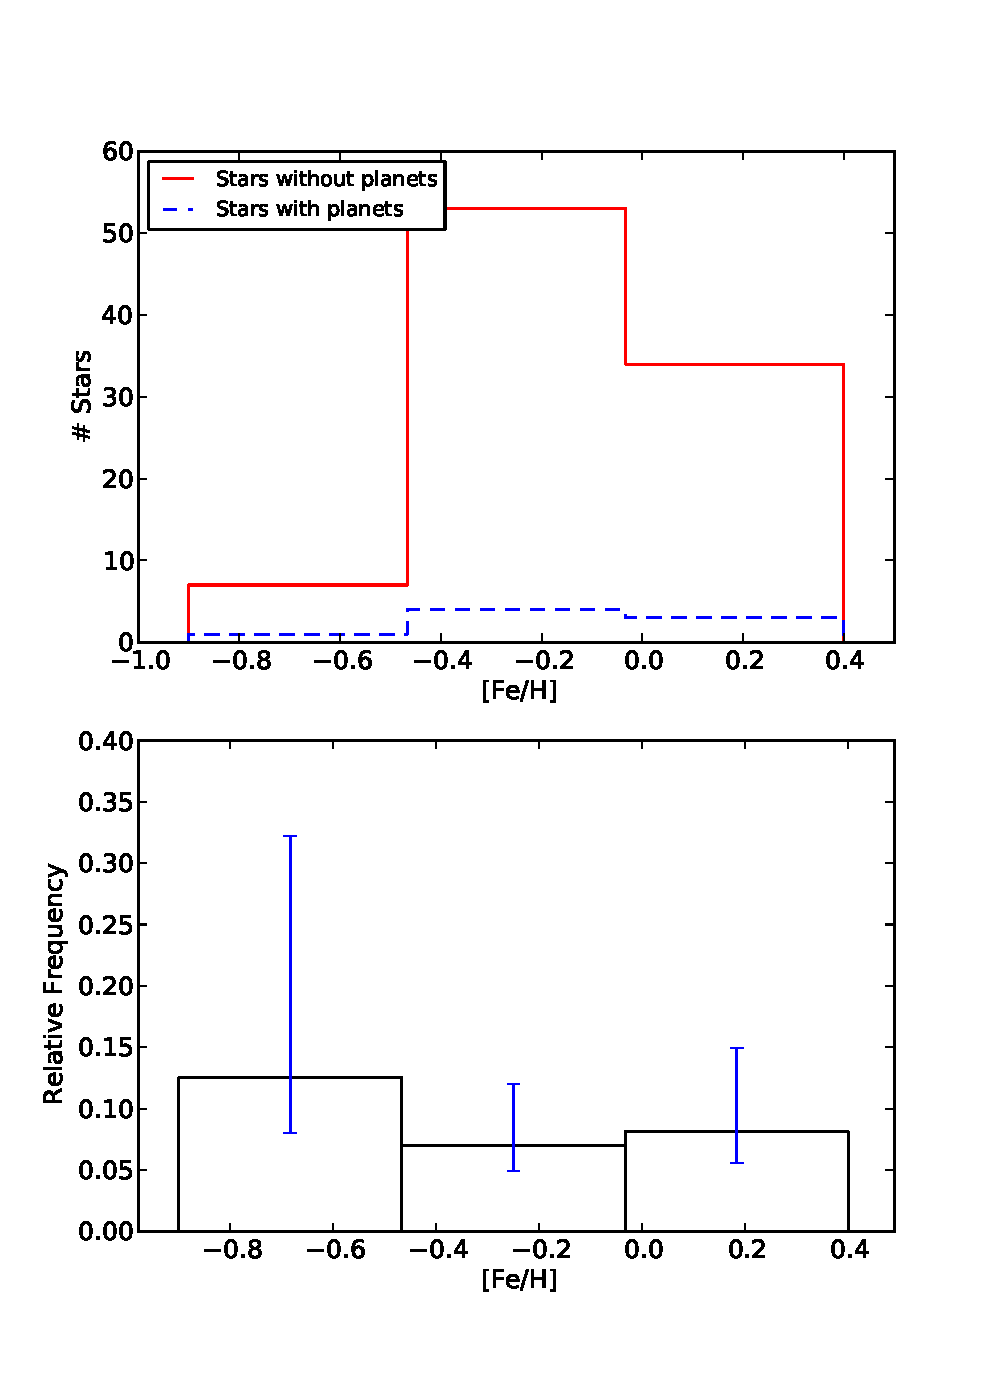
\includegraphics[scale=0.6]{../harpsm/all/pics_harpsmgtovpaper/3binfeh.eps}
\end{center}
\caption{Upper panel: Histogram of metallicity with 3 bins for stars without planets(solid red) and stars with planets (dashed blue); Lower panel: Frequency of stars with planets.}
\label{3binfeh}
\end{figure}

\begin{figure}[h]
\begin{center}
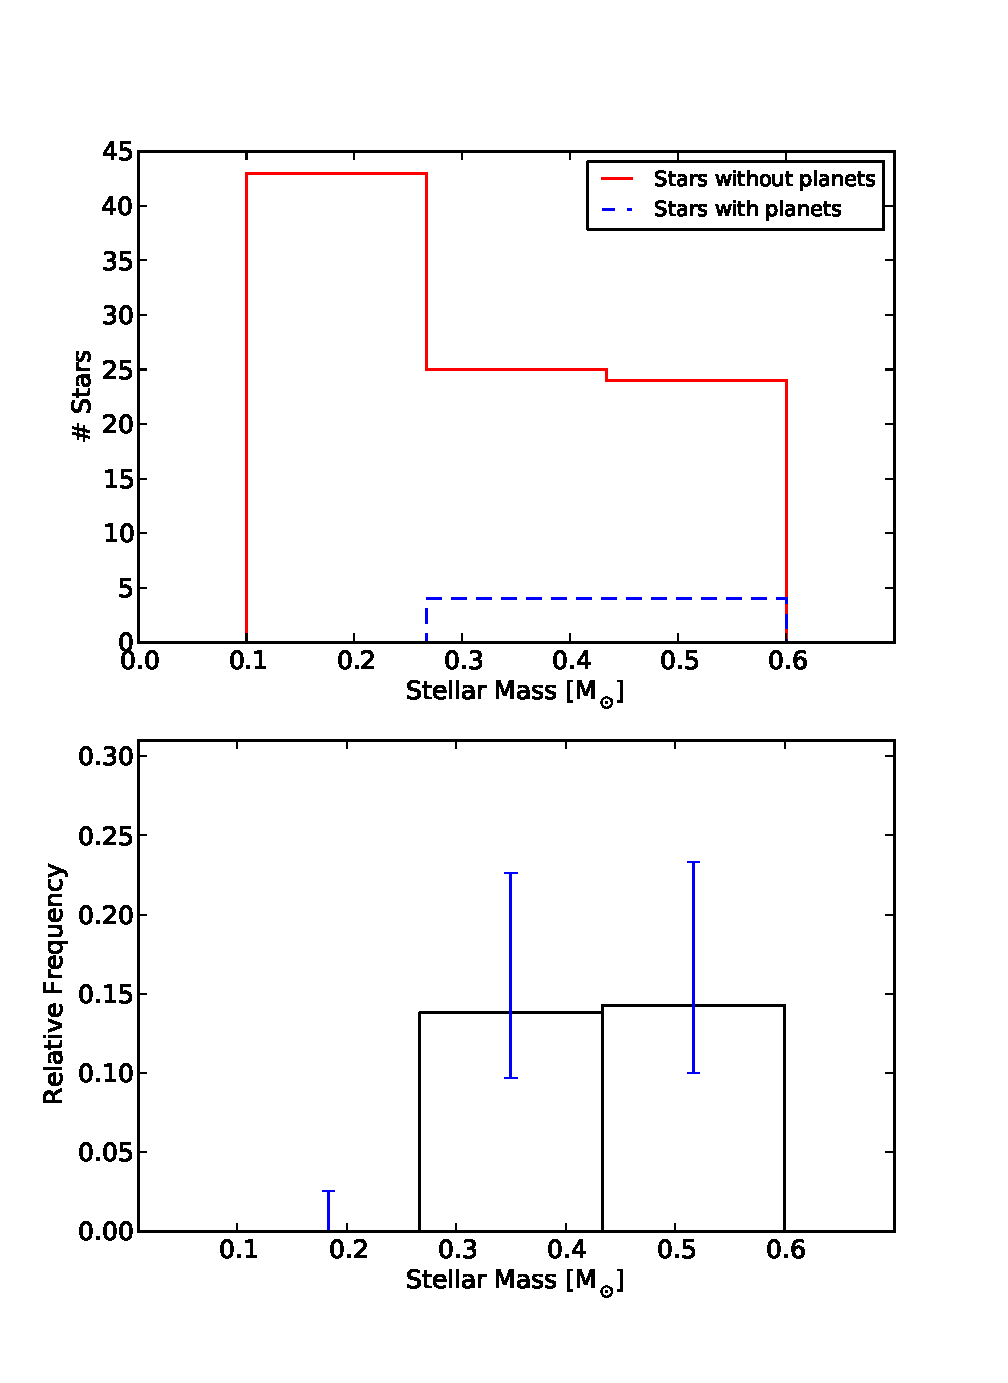
\includegraphics[scale=0.6]{../harpsm/all/pics_harpsmgtovpaper/3binmass.eps}
\end{center}
\caption{Upper panel: Histogram of stellar mass with 3 bins for stars without planets(solid red) and stars with planets (dashed blue); Lower panel: Frequency of stars with planets.}
\label{3binmass}
\end{figure}


The lower panels depict the relative frequency of the stars with planets. The errors in the frequency of each bin are calculated using the binomial distribution, 

\begin{equation}
P(f_{p},n,N) = \frac{N!}{n!(N-n)!}f^{n}_{p}(1-f_{p})^{N-n},
\label {binom}
\end{equation}
following the procedure outlined in, e.g., \citet[][]{Burgasser-2003,McCarthy-2004, Endl-2006}, and \citet{Sozzetti-2009}. \textbf{We calculate how many $n$ detections we have in a bin of size $N$, as a function of the planet frequency $f_{p}$, of each bin. Fig. \ref{binompdf} shows a normalized binomial probability distribution function with $n = 2$, $N = 20$, and $f_{p} = 0.1$. The upper errors, lower errors and upper limits of this assymetrical distribution are calculated by measuring the 68.2\% of the integrated area around the peak of the probability distribution function, that corresponds to the 1$\sigma$ limit for a gaussian distribution.} 

\begin{figure}[h]
\begin{center}
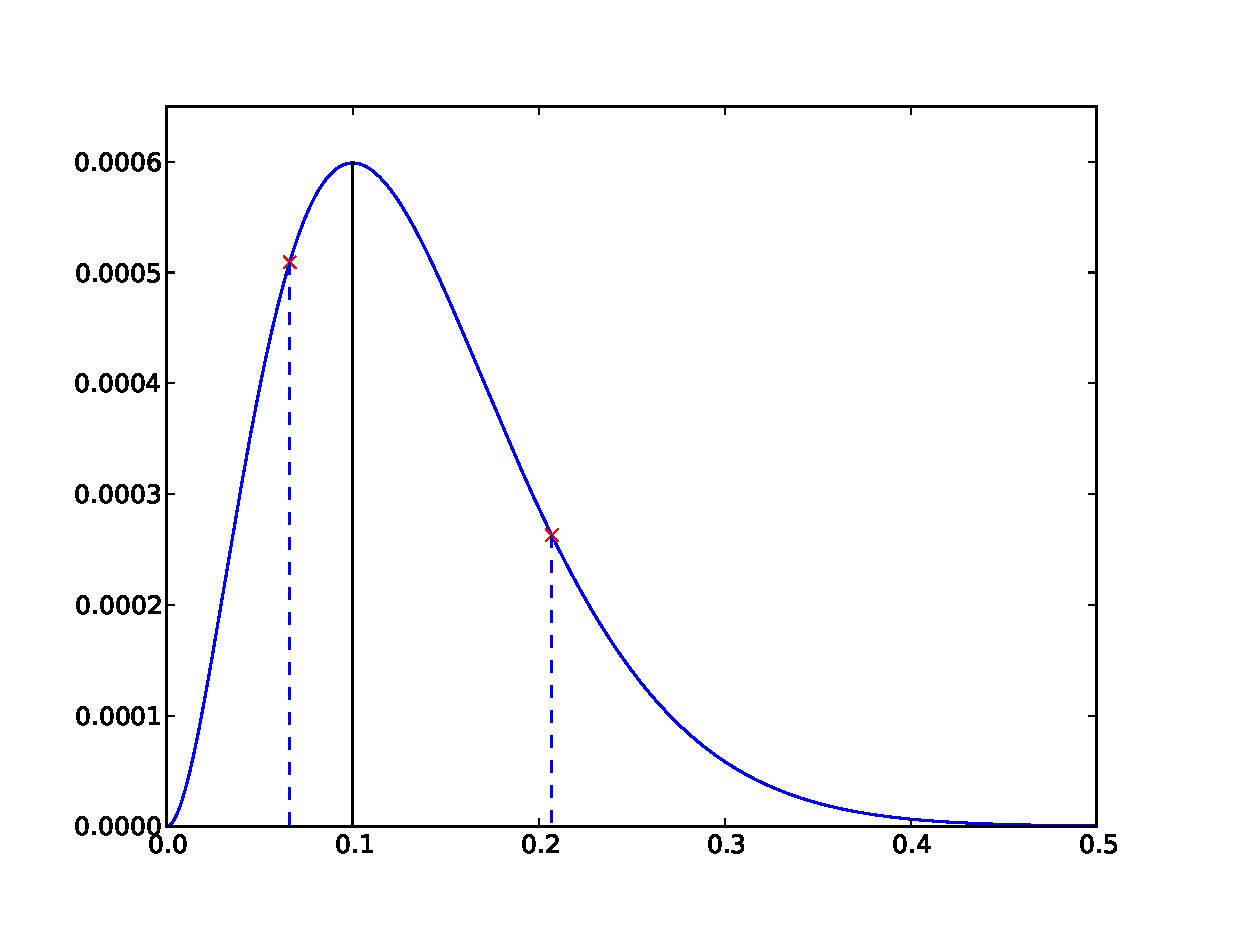
\includegraphics[scale=0.45]{../harpsm/all/pics_harpsmgtovpaper/binompdf.eps}
\end{center}
\caption{Normalized binomial probability distribution function for $n=2$, $N=20$, and $f_{p} = 0.1$.The solid vertical line depicts the observed frequency. The dashed lines show the 68.2\% ($1\sigma$) limits around the maximum of the function.}
\label{binompdf}
\end{figure}

Regarding the frequency of planet-host stars with metallicity, it can be clearly seen that there is no statistical difference between the bins. The first bin (]-0.9,0.5] dex) has one planet detection, with a planet frequency of 12.5\%, while the second and third [Fe/H] bins (]-0.5,-0.1] and ]-0.1,0.3] dex) have lower frequencies, 7.0\% and 8.1\% respectively. 


%, as, according to results obtained for FGK dwarfs, do not seem to correlate with metallicity \citep[e.g.][]{Sousa-2011b}.

For the frequency of planetary systems with stellar mass, there is a statistically significative difference ($> 3\sigma$)  between the first bin ( $0.1 < M_{\star} \le 0.27$ and the values of the two higher stellar mass bins (up to 0.6 M$_{star}$). We observe that the upper limit of the first bin ($0.10 < M_{\star} \le 0.27$), has a value of  2.6\% and the frequencies of the two higher stellar mass bins ($0.27 < M_{\star} \le 0.43$ and $0.43 < M_{\star} \le 0.60$) are 13.8\% and 14.3\% respectively.


Quantitatively, the upper limit (1$\sigma$) of the first bin has a value of 0.0256 while the lowest value that the second bin can reach is 0.0966. This translates into a 3.7 $\sigma$ difference \textcolor{red}{Is this correct?} between the values of the two bins, meaning that we can already see a trend of planet frequency with stellar mass, even with only 8 stars with planets. \textbf{However, as we will see in Sect. \ref{dl}, this correlation is due to a detection bias.}

%we still have to check if this result is physical or due to a detection bias. This will be done in . }

\textbf{To test the metallicity results we performed a parametric and bin-independent fitting of the data based on bayesian inference. We followed the \citet{Johnson-2010} approach, using two functional forms for the planet frequency, $f_{p1} = C$ and $f_{p2} = C10^{\alpha [Fe/H]}$, and choosing uniformly distributed priors for the parameters C and $\alpha$. Table \ref{bayes} summarizes our results. Column 1 shows the functional forms used and respective parameters, column 2 the uniform prior range, column 3 the most likely value for the fit parameters and column 4 the $1\sigma$ gaussian-equivalent confidence intervals.} 

\begin{table}[h]
\centering
\caption{Parameters of the two bayesian models. \textcolor{red}{To be updated!}}
\label{bayes}
\begin{center}
\resizebox{9cm}{!}{
\begin{tabular}{l c c c}

\hline
\hline
Parameters  & Uniform  & most likely  & $1\sigma$ confidence  \\
                     & Prior       & value & intervals  \\
\hline
$f_{p1} = C$ & &  & \\
C & (0.01,0.30) & 0.08 & $^{+0.03}_{-0.02}$ \\
\hline
$f_{p2} = C10^{\alpha[Fe/H]}$ & & & \\
C & (0.01,0.30) & 0.09 & 0.03 \\
$\alpha$ & (-2.0,4.0) & 0.30 & 0.69 \\
\hline
\hline
\end{tabular}
}
\end{center}
\end{table}

We note that the $\alpha$ value of the $f_{p} = C10^{\alpha [Fe/H]}$ functional form has large uncertainties. The $\alpha$ value here can easily accommodate both positive or negative values. In order to check which functional form is preferred we used a method of Bayesian model comparison, following Kass \& Raftery (1995) \textcolor{red}{reference!}. In short, we first calculate for both functional forms the total probability of the model conditioned on the data (the evidence) by integrating over the full parameter space. Computationally, in the case of uniformly distributed priors, we can calculate the evidence as  

\begin{equation}
P(d|f) = \frac{\sum{P(d|X)}}{length(X)},
\end{equation}
where the $P(d|X)$ is the likelihood, or the probability of the parameters X given d, the data, and $length(X)$ is the length of the full parameter space. Then, we calculate the Bayes factor that is just the ratio of the evidence of both functional forms, 

\begin{equation}
B_{f} = \frac{P(d|f_{p2})}{P(d|f_{p1})}.
\end{equation}
According to Kass \& Raftery (1995) \textcolor{red}{reference!} a $B_{f}$ value over 20 gives a \textit{strong} evidence that the model $f_{p1}$ is better at fitting the data than the $f_{p2}$ model. In our case we got a Bayes factor of 0.25 (\textcolor{red}{Update the Bfg!!!)} meaning that our constant model can fit the data better than the more complex model $f_{p2} = C10^{\alpha[Fe/H]}$. Therefore, at this time, the constant model is preferred.

Despite the results of the parametric approach, more detections are needed to test whether this non-correlation has a physical meaning or not, and to allow the calculation of the frequency of giant and smaller hosts separately: the non-correlations seems to be only reflecting the higher number of lower mass planet hosts.

\subsection{Comparison with the California Planet Survey late-K and M-type dwarf sample}

Here we want to compare our results to a similar sample regarding the difference between planet hosts and non-planet hosts only. The California Planet Survey (CPS) late-K and M-type dwarf sample (\textcolor{red}{REF! see Johnson-2010}) was chosen for this goal. It is a 152 star sample where 19 planets are already detected around 11 hosts (\textcolor{red}{Put a table here similar to Table1?}). The metallicities and stellar masses were calculated using the \citet{Johnson-2009} and the \citet{Delfosse-2000} calibration, respectively. We note that the \citet{Johnson-2009} [Fe/H] calibration has a dispersion around $\sim$ 0.2 dex and a systematic offset towards higher [Fe/H], as shown in \citet{Neves-2012}. The offset amounts to 0.14 dex when we compare the [Fe/H] of the CPS sample to our own sample. (\textcolor{red}{missing two tables here})

We calculated the difference of averages and medians between planet hosts and non-planet hosts in the same way as we did for our sample, as shown in Table \ref{planets}. Table \ref{planets:keck} shows the results. For metallicity, we observe a much higher difference of averages and medians when compared to our sample, but this only reflects the higher number of Jovian hosts of the CPS sample. The difference of averages and medians for Jupiter-type planets is higher than in our sample but is compatible with our results. For Neptunian-type hosts the difference of averages and medians are indistinguishable from the non-planet host sample. 

We also performed a KS test for [Fe/H] between the three planet-host subsamples, taking advantage of the higher number of stars with planets of the CPS sample, as shown in Table \ref{planets:keck}. It can be seen that there is a very low probability ($\sim$0.3\%) that the Jovian hosts and the stars without planets belong to the same distribution. For the case of Neptunian-hosts, however, the KS p-value is high ($\sim$97\%). Again, this result is expected from previous works on FGK dwarfs \citep[e.g.][]{Sousa-2011b} and M dwarfs \citep[e.g.][]{Rojas-Ayala-2012}. 

Regarding stellar mass, we do not see any trend. The difference of averages and medians between planet hosts and non-planet hosts is negligible. This results is apparently different from ours, but, in fact, they agree, because, as we will see in Sect. \ref{dl}, our result for stellar mass is biased.

\begin{table}[h]
\centering
\caption{Difference of averages and medians between planet host and non-planet host distributions for the CPS late-K and M-type dwarf sample.}
\label{planets:keck}
\begin{center}
\resizebox{9cm}{!}{
\begin{tabular}{l r r r}

\hline
\hline
[Fe/H] & Diff. of averages & Diff. of medians & KS test \\
 & [dex] & [dex] & \\
\hline
Full sample (N$_{h}$=11) & 0.17 & 0.20 & 0.0598\\
Jovians hosts (N$_{h}$=6) & 0.35 & 0.33 & 0.0032\\
Neptunian/smaller hosts (N$_{h}$=5) & -0.05 & -0.06 & 0.9728 \\
\hline
Stellar mass & Diff. of averages & Diff. of medians \\
 & [M$_{\odot}$] & [M$_{\odot}$] \\
Full sample (N$_{h}$=11)  & -0.05 & -0.03 & \\
Jovians hosts (N$_{h}$=6) & -0.05 & -0.06 \\
Neptunian/smaller hosts (N$_{h}$=5) & -0.04 & -0.02 \\

\hline
\hline
\end{tabular}
}
\end{center}
\end{table}

Figure \ref{3feh:keck} shows, it its upper panel, the histograms of non-planet hosts (solid red line) and stars with planets (dashed blue line) of the CPS sample, similar to Fig. \ref{3binfeh} of our sample. The lower panel depicts the frequency of planets of each bin. It is interesting to see that with the higher planet-host count we may start to see a build-up of Neptunian and smaller planet host stars at lower metallicities and, as we go towards higher [Fe/H] values we observe the well established [Fe/H]-Giant planet host relation \citep[e.g.][]{Santos-2004b,Fischer-2005}. We must be cautious, however, as the number of planet hosts is still small. The observed frequencies, ranging from 20.0\% to 5.1\% are compatible with the results obtained with our sample.

\begin{figure}[h]
\begin{center}
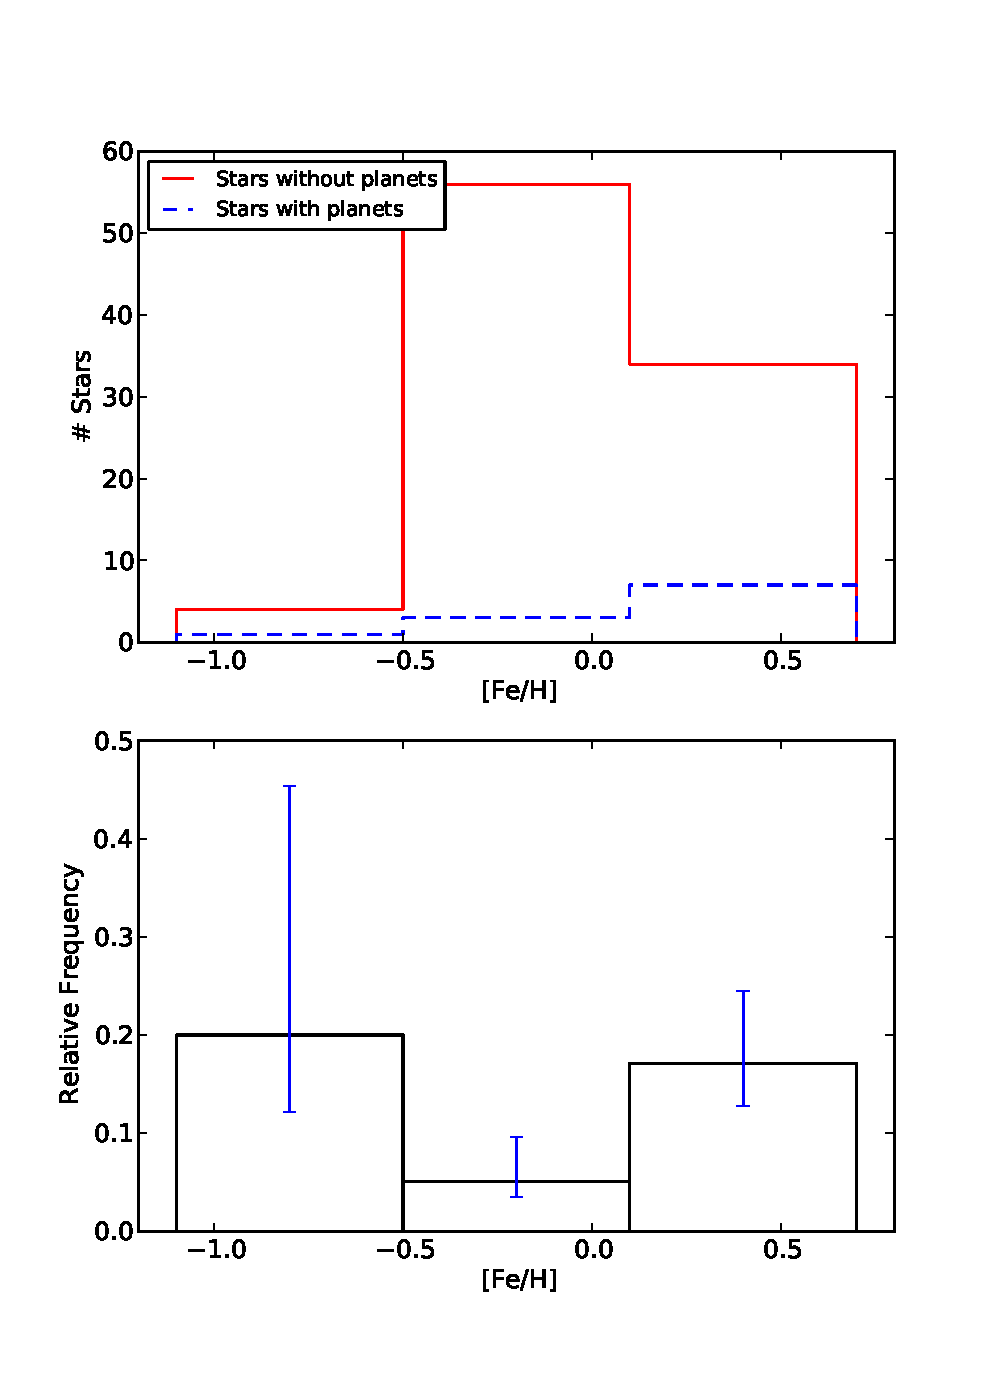
\includegraphics[scale=0.6]{../harpsm/all/pics_harpsmgtovpaper/3binfeh_keck.eps}
\end{center}
\caption{Upper panel: Histogram of metallicity with 3 bins for stars without planets(solid red) and stars with planets (dashed blue) for the CPS sample; Lower panel: Frequency of stars with planets.}
\label{3feh:keck}
\end{figure}



\section{Detection limits}
\label{dl}

In order to check if there is any statistically significative bias due to the detection limits \textbf{in the stellar mass distribution}, we will first investigate the reason why all planet detections of our sample are located in the brightest and more massive halves of the two distributions, as can be seen in Fig. \ref{histmass}, for the stellar mass (similar to Fig. 1 of \citet{Bonfils-2011}).

In order to do this, we divide the sample into two stellar mass ranges at the median value (0.29 M$_{\odot}$). We note that we removed the star Gl803 from the sample, due to the fact that the mass for this star may have not been adequately calculated, as explained in Sect. \ref{sample}. Then, we calculate, the frequency of stars with planets \textbf{(using only the most massive planet in stars with multiple planets)}, and the frequency of planets. For both cases, we take into account the detection limits of our sample for different regions of the mass-period diagram following the procedure described in Sect. 7 of \citet{Bonfils-2011}. 

\textbf{In short, for each region, we calculate the frequency $f=N_{d}/N_{\star,eff}$, where $N_{d}$ is the number of planet detections (or stars with planets), and $N_{\star,eff}$ is the number of stars whose detection limits exclude planets with similar mass and period at the 99\% confidence level. The N$_{\star,eff}$ is evaluated with Monte-Carlo sampling as described in \citet{Bonfils-2011}: we draw random mass and period within each region of study, assuming a log-uniform probability for both quantities. Then, we evaluate if the draw falls above or below the detection limit of each star. If it sits above the detection limit we include the star in the $N_{\star,eff}$. The final value of $N_{\star,eff}$ will be the average of 10.000 trials. The confidence intervals are calculated in a similar fashion as described in Sect. \ref{relation} but this time using a poissonian distribution to calculate the 1$\sigma$ gaussian-equivalent area of the probability distribution.}% limit equivalent confidence intervals.%, instead of using a binomial distribution. 

The results for the two halves of the stellar mass distribution can be seen in Table \ref{fswp} for the frequency of stars with planets (N=8), and in Table \ref{fpl} and for the occurrence of planets (N=14). We observe that, in the stars with planets case, all values between the upper limits for M$_{\star} \le $0.29M$_{\odot}$ and the frequency values  for M$_{\star} > $0.29M$_{\odot}$ are compatible with each other for all regions of planetary mass and period, except in the three regions with period between 10 and $10^{4}$ days, and mass between 1 and 10 M$_{\oplus}$, where we cannot compare the values due to a low N$_{eff}$ number. We observe the same regarding the results of the occurrence of planets. 

\textbf{The fact that we do not observe a statistically significative ($> 2\sigma$) difference in any region of the mass-period diagram between the two stellar mass samples means that the difference between the frequencies of the first two bins in Fig. \ref{3binmass} is not detected, when we take into account the detection limits.This indicates that the observed difference is due to a stellar mass detection bias. We need more detections to check if a real stellar mass trend exists or not.}

%Other than that, we cannot conclude anything regarding whether the observed stellar mass-planet dependence in Fig \ref{3binmass} is true or if it is just an observational bias towards brighter/ more massive stars.

\begin{table*}[t]
\begin{center}
\caption{a) Upper limits for the occurrence of stars with planets for M$_{\star} \leq 0.29$ $M_{\odot}$ (N$_{\star}$=52); b) Frequencies and upper limits for the occurrence of stars with planets for M$_{\star} > 0.29$ $M_{\odot}$ (N$_{\star}$=49). Multiplanetary systems are characterized by their most massive planet. }
\label{fswp}
\subtable[]{
\tiny
\resizebox{8.5cm}{!}{

\begin{tabular}{l | c c c c}
\hline
\hline

                &  \multicolumn{4}{c}{Period} \\
$m\sin{i}$ & \multicolumn{4}{c}{[day]} \\

\multicolumn{1}{c |}{[M$_{\oplus}$]}  & $1-10$ & $10 - 10^{2}$ & $10^{2} - 10^{3}$ & $10^{3} - 10^{4}$ \\
\hline
$10^3 - 10^4$ & $N_{d}=0$ & $N_{d}=0$ & $N_{d}=0$ & $N_{d}=0$ \\
              & $N_{eff} = 47.51$ & $N_{eff} = 46.85$ & $N_{eff} = 45.74$ & $N_{eff} = 42.67$ \\
              & $f<0.02(1\sigma)$ & $f<0.02(1\sigma)$ & $f<0.02(1\sigma)$ & $f<0.03(1\sigma)$ \\
$10^2 - 10^3$ & $N_{d}=0$ & $N_{d}=0$ & $N_{d}=0$ & $N_{d}=0$ \\
              & $N_{eff} = 44.11$ & $N_{eff} = 41.19$ & $N_{eff} = 36.31$ & $N_{eff} = 24.39$ \\
              & $f<0.03(1\sigma)$ & $f<0.03(1\sigma)$ & $f<0.03(1\sigma)$ & $f<0.05(1\sigma)$ \\
$10 - 10^2$ & $N_{d}=0$ & $N_{d}=0$ & $N_{d}=0$ & $N_{d}=0$ \\
              & $N_{eff} = 28.56$ & $N_{eff} = 18.86$ & $N_{eff} = 9.90$ & $N_{eff} = 3.43$ \\
              & $f<0.04(1\sigma)$ & $f<0.06(1\sigma)$ & $f<0.12(1\sigma)$ & $f<0.31(1\sigma)$ \\
$1 - 10$ & $N_{d}=0$ & $N_{d}=0$ & $N_{d}=0$ & $N_{d}=0$ \\
              & $N_{eff} = 3.90$ & $N_{eff} = 1.45$ & $N_{eff} = 0.46$ & $N_{eff} = 0.01$ \\
              & $f<0.28(1\sigma)$ & $ - $ & $ - $ & $ - $ \\ [1pt]

\hline
\hline
\end{tabular}}}
\subtable[]{
\tiny
\resizebox{8.35cm}{!}{
\begin{tabular}{l | c c c c}

%\caption{Frequencies and upper limits for the occurrence of stars with planets for M$_{\star} > 0.29$ $M_{\odot}$ (N$_{\star}$=49). Multiplanetary systems are characterized by their most massive planet.}




\hline
\hline

                &  \multicolumn{4}{c}{Period} \\
$m\sin{i}$ & \multicolumn{4}{c}{[day]} \\

\multicolumn{1}{c |}{[M$_{\oplus}$]}  & $1-10$ & $10 - 10^{2}$ & $10^{2} - 10^{3}$ & $10^{3} - 10^{4}$ \\
\hline
$10^3 - 10^4$ & $N_{d}=0$ & $N_{d}=0$ & $N_{d}=0$ & $N_{d}=0$ \\
              & $N_{eff} = 48.93$ & $N_{eff} = 48.73$ & $N_{eff} = 48.34$ & $N_{eff} = 47.24$ \\
              & $f<0.02(1\sigma)$ & $f<0.02(1\sigma)$ & $f<0.02(1\sigma)$ & $f<0.02(1\sigma)$ \\
$10^2 - 10^3$ & $N_{d}=0$ & $N_{d}=1$ & $N_{d}=0$ & $N_{d}=2$ \\
              & $N_{eff} = 47.79$ & $N_{eff} = 47.03$ & $N_{eff} = 44.74$ & $N_{eff} = 34.66$ \\
              & $f<0.02(1\sigma)$ & $f=0.02_{-0.01}^{+0.05}$ & $f<0.03(1\sigma)$ & $f=0.06_{-0.02}^{+0.08}$ \\
$10 - 10^2$ & $N_{d}=2$ & $N_{d}=0$ & $N_{d}=0$ & $N_{d}=0$ \\
              & $N_{eff} = 40.26$ & $N_{eff} = 31.78$ & $N_{eff} = 19.98$ & $N_{eff} = 7.18$ \\
              & $f=0.05_{-0.02}^{+0.07}$ & $f<0.04(1\sigma)$ & $f<0.06(1\sigma)$ & $f<0.16(1\sigma)$ \\
$1 - 10$ & $N_{d}=3$ & $N_{d}=0$ & $N_{d}=0$ & $N_{d}=0$ \\
              & $N_{eff} = 9.44$ & $N_{eff} = 3.89$ & $N_{eff} = 0.98$ & $N_{eff} = 0.10$ \\
              & $f=0.32_{-0.10}^{+0.31}$ & $f < 0.28 (1\sigma)$ & $ - $ & $ - $ \\ [1pt]
\hline
\hline
\end{tabular}}}
\end{center}
\end{table*}


%\begin{table}[h]
%\centering
%\caption{Upper limits for the occurrence of stars with planets for M$_{\star} \leq 0.29$ $M_{\odot}$ (N$_{\star}$=52). }
%\label{fswpl}
%\begin{center}
%\resizebox{9cm}{!}{
%\begin{tabular}{l | c c c c}
%
%\hline
%\hline
%
%                &  \multicolumn{4}{c}{Period} \\
%$m\sin{i}$ & \multicolumn{4}{c}{[day]} \\
%
%\multicolumn{1}{c |}{[M$_{\oplus}$]}  & $1-10$ & $10 - 10^{2}$ & $10^{2} - 10^{3}$ & $10^{3} - 10^{4}$ \\
%\hline
%$10^3 - 10^4$ & $N_{d}=0$ & $N_{d}=0$ & $N_{d}=0$ & $N_{d}=0$ \\
%              & $N_{eff} = 47.51$ & $N_{eff} = 46.85$ & $N_{eff} = 45.74$ & $N_{eff} = 42.67$ \\
%              & $f<0.02(1\sigma)$ & $f<0.02(1\sigma)$ & $f<0.02(1\sigma)$ & $f<0.03(1\sigma)$ \\
%$10^2 - 10^3$ & $N_{d}=0$ & $N_{d}=0$ & $N_{d}=0$ & $N_{d}=0$ \\
%              & $N_{eff} = 44.11$ & $N_{eff} = 41.19$ & $N_{eff} = 36.31$ & $N_{eff} = 24.39$ \\
%              & $f<0.03(1\sigma)$ & $f<0.03(1\sigma)$ & $f<0.03(1\sigma)$ & $f<0.05(1\sigma)$ \\
%$10 - 10^2$ & $N_{d}=0$ & $N_{d}=0$ & $N_{d}=0$ & $N_{d}=0$ \\
%              & $N_{eff} = 28.56$ & $N_{eff} = 18.86$ & $N_{eff} = 9.90$ & $N_{eff} = 3.43$ \\
%              & $f<0.04(1\sigma)$ & $f<0.06(1\sigma)$ & $f<0.12(1\sigma)$ & $f<0.31(1\sigma)$ \\
%$1 - 10$ & $N_{d}=0$ & $N_{d}=0$ & $N_{d}=0$ & $N_{d}=0$ \\
%              & $N_{eff} = 3.90$ & $N_{eff} = 1.45$ & $N_{eff} = 0.46$ & $N_{eff} = 0.01$ \\
%              & $f<0.28(1\sigma)$ & $ - $ & $ - $ & $ - $ \\ [1pt]
%
%\hline
%\hline
%\end{tabular}
%}
%\end{center}
%\end{table}
%
%\begin{table}[h]
%\centering
%\caption{Frequencies and upper limits for the occurrence of stars with planets for M$_{\star} > 0.29$ $M_{\odot}$ (N$_{\star}$=49). Multiplanetary systems are characterized by their most massive planet.}
%\label{fswpu}
%\begin{center}
%\resizebox{9cm}{!}{
%\begin{tabular}{l | c c c c}
%
%\hline
%\hline
%
%                &  \multicolumn{4}{c}{Period} \\
%$m\sin{i}$ & \multicolumn{4}{c}{[day]} \\
%
%\multicolumn{1}{c |}{[M$_{\oplus}$]}  & $1-10$ & $10 - 10^{2}$ & $10^{2} - 10^{3}$ & $10^{3} - 10^{4}$ \\
%\hline
%$10^3 - 10^4$ & $N_{d}=0$ & $N_{d}=0$ & $N_{d}=0$ & $N_{d}=0$ \\
%              & $N_{eff} = 48.93$ & $N_{eff} = 48.73$ & $N_{eff} = 48.34$ & $N_{eff} = 47.24$ \\
%              & $f<0.02(1\sigma)$ & $f<0.02(1\sigma)$ & $f<0.02(1\sigma)$ & $f<0.02(1\sigma)$ \\
%$10^2 - 10^3$ & $N_{d}=0$ & $N_{d}=1$ & $N_{d}=0$ & $N_{d}=2$ \\
%              & $N_{eff} = 47.79$ & $N_{eff} = 47.03$ & $N_{eff} = 44.74$ & $N_{eff} = 34.66$ \\
%              & $f<0.02(1\sigma)$ & $f=0.02_{-0.01}^{+0.05}$ & $f<0.03(1\sigma)$ & $f=0.06_{-0.02}^{+0.08}$ \\
%$10 - 10^2$ & $N_{d}=2$ & $N_{d}=0$ & $N_{d}=0$ & $N_{d}=0$ \\
%              & $N_{eff} = 40.26$ & $N_{eff} = 31.78$ & $N_{eff} = 19.98$ & $N_{eff} = 7.18$ \\
%              & $f=0.05_{-0.02}^{+0.07}$ & $f<0.04(1\sigma)$ & $f<0.06(1\sigma)$ & $f<0.16(1\sigma)$ \\
%$1 - 10$ & $N_{d}=3$ & $N_{d}=0$ & $N_{d}=0$ & $N_{d}=0$ \\
%              & $N_{eff} = 9.44$ & $N_{eff} = 3.89$ & $N_{eff} = 0.98$ & $N_{eff} = 0.10$ \\
%              & $f=0.32_{-0.10}^{+0.31}$ & $f < 0.28 (1\sigma)$ & $ - $ & $ - $ \\ [1pt]
%\hline
%\hline
%\end{tabular}
%}
%\end{center}
%\end{table}

\begin{table*}[t]
%\centering
\begin{center}
\caption{a) Upper limits for the occurrence of planets for M$_{\star} \leq 0.29$ $M_{\odot}$ (N$_{\star}$=52); b) Frequencies and upper limits for the occurrence of planets for M$_{\star} > 0.29$ $M_{\odot}$ (N$_{\star}$=49).   }
\label{fpl}
\subtable[]{
\tiny
\resizebox{8.5cm}{!}{
\begin{tabular}{l | c c c c}

\hline
\hline

                &  \multicolumn{4}{c}{Period} \\
$m\sin{i}$ & \multicolumn{4}{c}{[day]} \\

\multicolumn{1}{c |}{[M$_{\oplus}$]}  & $1-10$ & $10 - 10^{2}$ & $10^{2} - 10^{3}$ & $10^{3} - 10^{4}$ \\
\hline
$10^3 - 10^4$ & $N_{d}=0$ & $N_{d}=0$ & $N_{d}=0$ & $N_{d}=0$ \\
              & $N_{eff} = 47.51$ & $N_{eff} = 46.85$ & $N_{eff} = 45.74$ & $N_{eff} = 42.70$ \\
              & $f<0.02(1\sigma)$ & $f<0.02(1\sigma)$ & $f<0.02(1\sigma)$ & $f<0.03(1\sigma)$ \\
$10^2 - 10^3$ & $N_{d}=0$ & $N_{d}=0$ & $N_{d}=0$ & $N_{d}=0$ \\
              & $N_{eff} = 44.13$ & $N_{eff} = 41.24$ & $N_{eff} = 36.45$ & $N_{eff} = 24.63$ \\
              & $f<0.03(1\sigma)$ & $f<0.03(1\sigma)$ & $f<0.03(1\sigma)$ & $f<0.05(1\sigma)$ \\
$10 - 10^2$ & $N_{d}=0$ & $N_{d}=0$ & $N_{d}=0$ & $N_{d}=0$ \\
              & $N_{eff} = 28.51$ & $N_{eff} = 18.84$ & $N_{eff} = 9.89$ & $N_{eff} = 3.46$ \\
              & $f<0.04(1\sigma)$ & $f<0.06(1\sigma)$ & $f<0.12(1\sigma)$ & $f<0.31(1\sigma)$ \\
$1 - 10$ & $N_{d}=0$ & $N_{d}=0$ & $N_{d}=0$ & $N_{d}=0$ \\
              & $N_{eff} = 3.92$ & $N_{eff} = 1.47$ & $N_{eff} = 0.47$ & $N_{eff} = 0.01$ \\
              & $f<0.28(1\sigma)$ & $ - $ & $ - $ & $ - $ \\ [1pt]
\hline
\hline
\end{tabular}}}
\subtable[][]{
\tiny
\resizebox{8.35cm}{!}{
\begin{tabular}{l | c c c c}

\hline
\hline

                &  \multicolumn{4}{c}{Period} \\
$m\sin{i}$ & \multicolumn{4}{c}{[day]} \\

\multicolumn{1}{c |}{[M$_{\oplus}$]}  & $1-10$ & $10 - 10^{2}$ & $10^{2} - 10^{3}$ & $10^{3} - 10^{4}$ \\
\hline
$10^3 - 10^4$ & $N_{d}=0$ & $N_{d}=0$ & $N_{d}=0$ & $N_{d}=0$ \\
              & $N_{eff} = 48.92$ & $N_{eff} = 48.71$ & $N_{eff} = 48.34$ & $N_{eff} = 47.21$ \\
              & $f<0.02(1\sigma)$ & $f<0.02(1\sigma)$ & $f<0.02(1\sigma)$ & $f<0.02(1\sigma)$ \\
$10^2 - 10^3$ & $N_{d}=0$ & $N_{d}=2$ & $N_{d}=0$ & $N_{d}=2$ \\
              & $N_{eff} = 47.78$ & $N_{eff} = 47.02$ & $N_{eff} = 44.65$ & $N_{eff} = 34.48$ \\
              & $f<0.02(1\sigma)$ & $f=0.04_{-0.01}^{+0.06}$ & $f<0.03(1\sigma)$ & $f=0.06_{-0.02}^{+0.08}$ \\
$10 - 10^2$ & $N_{d}=2$ & $N_{d}=0$ & $N_{d}=1$ & $N_{d}=1$ \\
              & $N_{eff} = 40.23$ & $N_{eff} = 31.60$ & $N_{eff} = 19.85$ & $N_{eff} = 7.05$ \\
              & $f=0.05_{-0.02}^{+0.07}$ & $f<0.04(1\sigma)$ & $f=0.05_{-0.01}^{+0.12}$ & $f=0.14_{-0.04}^{+0.33}$ \\
$1 - 10$ & $N_{d}=5$ & $N_{d}=3$ & $N_{d}=0$ & $N_{d}=0$ \\
              & $N_{eff} = 9.46$ & $N_{eff} = 3.90$ & $N_{eff} = 0.99$ & $N_{eff} = 0.10$ \\
              & $f=0.53_{-0.15}^{+0.36}$ & $f=0.77_{-0.23}^{+0.75}$ & $ - $ & $ - $ \\ [1pt]

\hline
\hline
\end{tabular}}}

\end{center}
\end{table*}


%\begin{table}[]
%\centering
%\caption{Upper limits for the occurrence of planets for M$_{\star} \leq 0.29$ $M_{\odot}$ (N$_{\star}$=52).   }
%\label{fpl}
%\begin{center}
%\resizebox{9cm}{!}{
%\begin{tabular}{l | c c c c}
%
%\hline
%\hline
%
%                &  \multicolumn{4}{c}{Period} \\
%$m\sin{i}$ & \multicolumn{4}{c}{[day]} \\
%
%\multicolumn{1}{c |}{[M$_{\oplus}$]}  & $1-10$ & $10 - 10^{2}$ & $10^{2} - 10^{3}$ & $10^{3} - 10^{4}$ \\
%\hline
%$10^3 - 10^4$ & $N_{d}=0$ & $N_{d}=0$ & $N_{d}=0$ & $N_{d}=0$ \\
%              & $N_{eff} = 47.51$ & $N_{eff} = 46.85$ & $N_{eff} = 45.74$ & $N_{eff} = 42.70$ \\
%              & $f<0.02(1\sigma)$ & $f<0.02(1\sigma)$ & $f<0.02(1\sigma)$ & $f<0.03(1\sigma)$ \\
%$10^2 - 10^3$ & $N_{d}=0$ & $N_{d}=0$ & $N_{d}=0$ & $N_{d}=0$ \\
%              & $N_{eff} = 44.13$ & $N_{eff} = 41.24$ & $N_{eff} = 36.45$ & $N_{eff} = 24.63$ \\
%              & $f<0.03(1\sigma)$ & $f<0.03(1\sigma)$ & $f<0.03(1\sigma)$ & $f<0.05(1\sigma)$ \\
%$10 - 10^2$ & $N_{d}=0$ & $N_{d}=0$ & $N_{d}=0$ & $N_{d}=0$ \\
%              & $N_{eff} = 28.51$ & $N_{eff} = 18.84$ & $N_{eff} = 9.89$ & $N_{eff} = 3.46$ \\
%              & $f<0.04(1\sigma)$ & $f<0.06(1\sigma)$ & $f<0.12(1\sigma)$ & $f<0.31(1\sigma)$ \\
%$1 - 10$ & $N_{d}=0$ & $N_{d}=0$ & $N_{d}=0$ & $N_{d}=0$ \\
%              & $N_{eff} = 3.92$ & $N_{eff} = 1.47$ & $N_{eff} = 0.47$ & $N_{eff} = 0.01$ \\
%              & $f<0.28(1\sigma)$ & $ - $ & $ - $ & $ - $ \\ [1pt]
%\hline
%\hline
%\end{tabular}
%}
%\end{center}
%\end{table}
%
%\begin{table}[]
%\centering
%\caption{Frequencies and upper limits for the occurrence of planets for M$_{\star} > 0.29$ $M_{\odot}$ (N$_{\star}$=49).    }
%\label{fpu}
%\begin{center}
%\resizebox{9cm}{!}{
%\begin{tabular}{l | c c c c}
%
%\hline
%\hline
%
%                &  \multicolumn{4}{c}{Period} \\
%$m\sin{i}$ & \multicolumn{4}{c}{[day]} \\
%
%\multicolumn{1}{c |}{[M$_{\oplus}$]}  & $1-10$ & $10 - 10^{2}$ & $10^{2} - 10^{3}$ & $10^{3} - 10^{4}$ \\
%\hline
%$10^3 - 10^4$ & $N_{d}=0$ & $N_{d}=0$ & $N_{d}=0$ & $N_{d}=0$ \\
%              & $N_{eff} = 48.92$ & $N_{eff} = 48.71$ & $N_{eff} = 48.34$ & $N_{eff} = 47.21$ \\
%              & $f<0.02(1\sigma)$ & $f<0.02(1\sigma)$ & $f<0.02(1\sigma)$ & $f<0.02(1\sigma)$ \\
%$10^2 - 10^3$ & $N_{d}=0$ & $N_{d}=2$ & $N_{d}=0$ & $N_{d}=2$ \\
%              & $N_{eff} = 47.78$ & $N_{eff} = 47.02$ & $N_{eff} = 44.65$ & $N_{eff} = 34.48$ \\
%              & $f<0.02(1\sigma)$ & $f=0.04_{-0.01}^{+0.06}$ & $f<0.03(1\sigma)$ & $f=0.06_{-0.02}^{+0.08}$ \\
%$10 - 10^2$ & $N_{d}=2$ & $N_{d}=0$ & $N_{d}=0$ & $N_{d}=0$ \\
%              & $N_{eff} = 40.23$ & $N_{eff} = 31.60$ & $N_{eff} = 19.75$ & $N_{eff} = 7.07$ \\
%              & $f=0.05_{-0.02}^{+0.07}$ & $f<0.04(1\sigma)$ & $f<0.06(1\sigma)$ & $f<0.16(1\sigma)$ \\
%$1 - 10$ & $N_{d}=5$ & $N_{d}=3$ & $N_{d}=0$ & $N_{d}=0$ \\
%              & $N_{eff} = 9.46$ & $N_{eff} = 3.90$ & $N_{eff} = 0.99$ & $N_{eff} = 0.10$ \\
%              & $f=0.53_{-0.15}^{+0.36}$ & $f=0.77_{-0.23}^{+0.75}$ & $ - $ & $ - $ \\ [1pt]
%
%\hline
%\hline
%\end{tabular}
%}
%\end{center}
%\end{table}
 

\textbf{We got similar results for the V magnitude distribution. The V-mag and stellar mass have similar effects, as the stellar mass increases linearly with the visual magnitude.}













\section{Discussion}
\label{discussion}

\textbf{In this paper we investigate the metallicity and stellar mass correlations with planets. We use a new method, described in the Appendix, to refine the precision of the metallicities calculated with the calibration of \citet{Neves-2012}. We use the established calibration of \citet{Delfosse-2000} to calculate the stellar masses of our sample.} % based on the photometric calibration of \citet{Neves-2012}, itself a refinement of the \citet{Schlaufman-2010} calibration.} 
\textcolor{red}{why did you strikeout 'investigate'?}

We do not detect a trend of metallicity with the presence of planets. We attribute this non-correlation to the fact that we only have 3 planet-host stars with Jupiter-type planets. The frequency of planets sits between 12.5 and 7.0 \% for the sample [Fe/H] range, between -0.88 and 0.32 dex. The uncertainties associated to these frequencies are still high, due to the small number of planet hosts in our sample.

An alternative method to the binning approach, based on Bayesian inference, was also used to test the metallicity frequency results. We investigated two functional forms, $f_{p1} = C$ and $f_{p2} = C10^{\alpha[Fe/H]}$, and concluded that the constant model with $f_{p} = 8.0\%$  is preferred over the more complex model. 

We calculated the difference of the averages and medians between planet-host and non-planet-host distributions. A significative difference emerges for Jupiter-type hosts where the difference of the averages and the medians is 0.20 and 0.26 dex respectively. This result is in line with previous works \citep[e.g.][]{Bonfils-2007,Johnson-2009, Schlaufman-2010, Rojas-Ayala-2012, Terrien-2012}.Regarding the Neptunian and smaller planet hosts, the observed difference of the averages and the medians is -0.10 dex, agreeing with the results for Neptunian-type planets orbiting FGK-type dwarfs \citep[e.g][]{Sousa-2011b, Mayor-2011} and M dwarfs \citep[e.g.][]{Rojas-Ayala-2012,Terrien-2012}. In fact, the result for Neptunians and smaller hosts hint at an anti-correlation of [Fe/H] with planets, but the result is at the precision limit of our metallicity technique. 

We note that we only have 8 planet hosts in our sample. Therefore we should consider the results as hints, that need more detections to be confirmed as true trends.

Regarding stellar mass, we detect a significant ($>3\sigma$) positive trend in the planet host frequency histogram. However, when we take the detection limits into account, we do not find any significant difference. Therefore, the trend of the frequency of planets with the stellar mass is due to a detection bias in our sample, stressing the importance of taking into account the planet detection biases in stellar mass studies.

%Despite that, we need more detections to robustly confirm whether there is a true stellar mass trend or not.


%In this work, we derive the metallicities of a sample of 102 M dwarfs from the HARPS GTO programme. We use a new method, using the high-resolution spectra of HARPS, described in the Appendix, to refine and enhance the precision of metallicities based on the photometric calibration of \citet{Neves-2012}, itself a refinement of the \citet{Schlaufman-2010} calibration. Then, we use this determinations, as well as stellar mass determinations from \citet{Bonfils-2011}, calculated using the mass-luminosity relation of \citet{Delfosse-2000} to search for correlation between the frequency of planets and stellar mass and metallicity. In Sect. \ref{sample}, we describe the sample of M dwarfs and the observations using the HARPS spectrograph. Then, in Sect. \ref{relation}, we investigate the stellar mass/metallcity correlations with the frequency of planets. Afterwards, we calculate the detection limits of the sample, to check for biases in our sample, since the planet detections accumulate in the higher end of stellar mass and lower end of V magnitude. Finally, we discuss our results in Sect. \ref{discussion}.





\begin{acknowledgements}
We would like to thank A. Mortier for useful discussions. We acknowledge the
support by the European Research Council/European Community under the
FP7 through Starting Grant agreement number 239953. NCS and VN also
acknowledges the support from Funda\c{c}\~ao para a Ci\^encia e a
Tecnologia (FCT) through program Ci\^encia\,2007 funded by FCT/MCTES
(Portugal) and POPH/FSE (EC), and in the form of grant reference
PTDC/CTE-AST/098528/2008. VN would also like to acknowledge the
support from the FCT in the form of the fellowship SFRH/BD/60688/2009. 
\textcolor{red}{PUT sinbad and 2mass in the acknowledgements e perguntar ao NUNO para ver os acknowledgements (ciencia 2007?)}      


\end{acknowledgements}

\bibliographystyle{aa}
\bibliography{mylib.bib}

\appendix

\label{appendix}

\section{A new M dwarf metallicity and effective temperature calibration based on line and feature measurements of HARPS M dwarf spectra}

Here we briefly explain the method that we developed to estimate the metallicity and effective temperature of M dwarfs. \textbf{A paper regarding the full details of this calibration is in preparation (Neves et al., in prep.).}

\textbf{The main goal of the new calibration is to investigate the metallicity difference between stars with and without planets. The method is based on the measurement of `peak-to-peak' equivalent widths (EW) of lines and features from the spectra of our volume-limited M dwarf HARPS sample and uses existing photometric calibrations for metallicity \citep{Neves-2012}  and effective temperature \citep{Casagrande-2008}, as starting values. Our method achieves an increase in precision of the metallicity and effective temperature but the accuracy of the new scale is tied to the accuracy of the photometric calibrations.}



%The \citet{Neves-2012} scale is a refinement of the the \citet{Sc}



%This scale is based on the metallicity photometric calibration of \citet{Neves-2012} (being itself a slight refinement of the one of \citet{Schlaufman-2010}) and the effective temperature calibration of \citet{Casagrande-2008}. %Therefore, we're solely improving the precision of the existing photometric calibration with the aid of measurements of lines and features of M dwarf spectra. 

\subsection{Calibration sample}

From the initial 102 M dwarf star spectra of the \citet{Bonfils-2011} sample we initially chose 60 stars with S/N greater than 100. Six stars (Gl191, Gl285, Gl388, Gl699, Gl729, Gl803, GJ1125) were then discarded \textit{a posteriori}, either due to high activity and high rotation of the star (that translates into a bad correlation of the line measurements with either the reference metallicity or temperature scales), or due to a bad value of the radial velocity (GJ1125). We ended up with a sample of 56 stars, shown in Table \ref{caltable} in which we based our calibration. Column 1 shows the star designation, column 2 the initial photometric [Fe/H], column 3 the calibrated [Fe/H] value, column 4 the initial photometric effective temperature, and column 5 the calibrated $T_{eff}$ value.

\begin{table}[]
\centering
\caption{Calibration sample.}
\label{caltable}
\begin{center}
%\resizebox{9cm}{!}{
\begin{tabular}{l r r r r }

\hline
\hline

star & [Fe/H]$_{N12}$ & [Fe/H]$_{NEW}$ & $T_{eff~C08}$ & $T_{eff~NEW}$ \\

\hline

Gl465 & -0.56 & -0.65 & 3365 & 3397 \\
Gl438 & -0.51 & -0.39 & 3506 & 3466 \\
Gl667C & -0.51 & -0.54 & 3460 & 3390 \\
Gl54.1 & -0.46 & -0.41 & 2920 & 3033 \\
Gl887 & -0.36 & -0.24 & 3657 & 3497 \\
Gl1 & -0.37 & -0.45 & 3495 & 3541 \\
Gl908 & -0.37 & -0.44 & 3579 & 3501 \\
Gl357 & -0.33 & -0.34 & 3329 & 3331 \\
Gl686 & -0.31 & -0.37 & 3536 & 3464 \\
Gl87 & -0.30 & -0.31 & 3539 & 3522 \\
Gl447 & -0.28 & -0.18 & 2958 & 3020 \\
Gl693 & -0.28 & -0.30 & 3178 & 3217 \\
Gl213 & -0.25 & -0.11 & 3062 & 3025 \\
Gl674 & -0.22 & -0.25 & 3276 & 3313 \\
LP771-95A & -0.09 & -0.34 & 3028 & 3212 \\
Gl832 & -0.18 & -0.19 & 3426 & 3454 \\
Gl701 & -0.19 & -0.27 & 3498 & 3477 \\
Gl536 & -0.16 & -0.12 & 3542 & 3526 \\
HIP31292 & -0.15 & -0.09 & 3156 & 3125 \\
Gl105B & -0.14 & -0.02 & 3057 & 2948 \\
Gl341 & -0.15 & -0.12 & 3606 & 3565 \\
Gl273 & -0.13 & -0.01 & 3119 & 3083 \\
Gl581 & -0.17 & -0.21 & 3186 & 3213 \\
Gl526 & -0.15 & -0.20 & 3503 & 3527 \\
Gl433 & -0.15 & -0.17 & 3453 & 3471 \\
GJ2066 & -0.11 & -0.18 & 3372 & 3432 \\
Gl678.1A & -0.13 & -0.11 & 3628 & 3562 \\
Gl413.1 & -0.11 & -0.12 & 3388 & 3387 \\
Gl618A & -0.08 & -0.08 & 3231 & 3247 \\
Gl393 & -0.10 & -0.22 & 3346 & 3422 \\
Gl514 & -0.10 & -0.16 & 3515 & 3534 \\
Gl250B & -0.09 & -0.10 & 3352 & 3390 \\
Gl628 & -0.06 & -0.02 & 3091 & 3050 \\
Gl367 & -0.05 & -0.07 & 3379 & 3385 \\
Gl229 & -0.04 & -0.00 & 3532 & 3633 \\
Gl846 & -0.06 & 0.06 & 3628 & 3609 \\
Gl680 & -0.04 & -0.22 & 3355 & 3415 \\
Gl752A & -0.00 & 0.06 & 3328 & 3352 \\
Gl877 & -0.02 & -0.01 & 3257 & 3279 \\
HIP31293 & 0.01 & -0.04 & 3236 & 3275 \\
Gl569A & 0.00 & -0.09 & 3327 & 3304 \\
Gl588 & 0.03 & 0.07 & 3277 & 3298 \\
Gl205 & -0.01 & 0.22 & 3576 & 3698 \\
Gl358 & 0.04 & -0.01 & 3194 & 3175 \\
Gl551 & 0.07 & -0.00 & 2625 & 2672 \\
Gl176 & 0.03 & -0.01 & 3344 & 3364 \\
Gl382 & 0.05 & 0.04 & 3397 & 3409 \\
Gl300 & 0.06 & 0.14 & 2973 & 2827 \\
Gl479 & 0.06 & 0.01 & 3219 & 3211 \\
Gl880 & 0.08 & 0.07 & 3453 & 3578 \\
Gl682 & 0.10 & 0.11 & 2973 & 2892 \\
Gl555 & 0.11 & 0.17 & 2983 & 2832 \\
Gl876 & 0.14 & 0.15 & 3036 & 2946 \\
LTT9759 & 0.16 & 0.21 & 3317 & 3313 \\
Gl849 & 0.23 & 0.24 & 3170 & 3129 \\

\hline
\hline
\end{tabular}
%}
\end{center}
\end{table}







\subsection{Method}

From our calibration sample we first measured `peak-to-peak' equivalent widths (EWs) of lines and features using the 26 redder orders of median normalized HARPS spectra, in the region between 530 to 690 nm. Here we consider features as blended lines. We define the `peak-to-peak' equivalent widths as

\begin{equation}
W = \sum{\frac{F_{pp}-F_{\lambda}}{F_{pp}}d\lambda},
\label{ew}
\end{equation}
where $F_{pp}$ is the value of the flux between the peaks of the line/feature at each integration step and $F_{\lambda}$ the flux of the line/feature. The measurement of the EWs is illustrated in Fig. \ref{spec}, where the `peak-to-peak' flux corresponds to the red dotted lines, and the black line is the flux of the reference spectra. The EW is thus measured between the red dotted line and the solid black line.  \textbf{We used the very high S/N ($\sim$1430 @ 550nm) spectral orders of the star Gl 209 as a reference from where the line/feature regions are going to be measured for all other stars. We rejected lines/features with EW $<$ 8 $m\AA$ and very steep lines/features.(\textcolor{red}{elaborate here?})}.

\begin{figure}[h]
\begin{center}
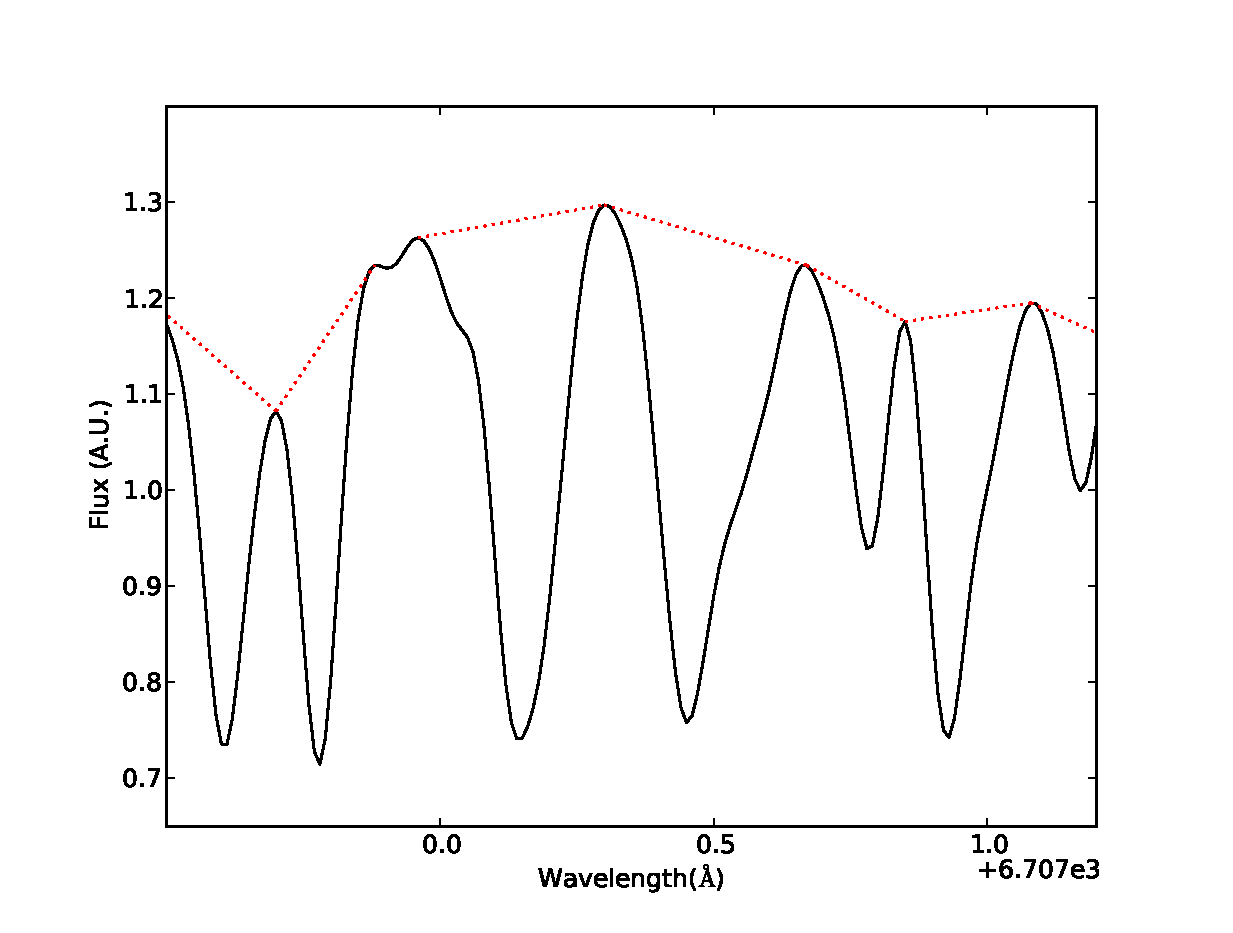
\includegraphics[scale=0.45]{../harpsm/all/pics_harpsmgtovpaper/template.eps}
\end{center}
\caption{Small region of the Gl 209 spectra illustrating the 'peak to peak' equivalent width line measurement.}
\label{spec}
\end{figure}


 \textbf{We investigated the correlations and partial correlations of [Fe/H] and $T_{eff}$ with the line/feature EWs. Fig. \ref{pcorr} shows the histograms of the partial correlation values of [Fe/H] with $T_{eff}$ kept constant(solid blue histogram) and the partial correlation values of $T_{eff}$ with [Fe/H] kept constant (dashed green histogram). We observe that a significant number of lines have a good correlation with the parameters.}

\begin{figure}[h]
\begin{center}
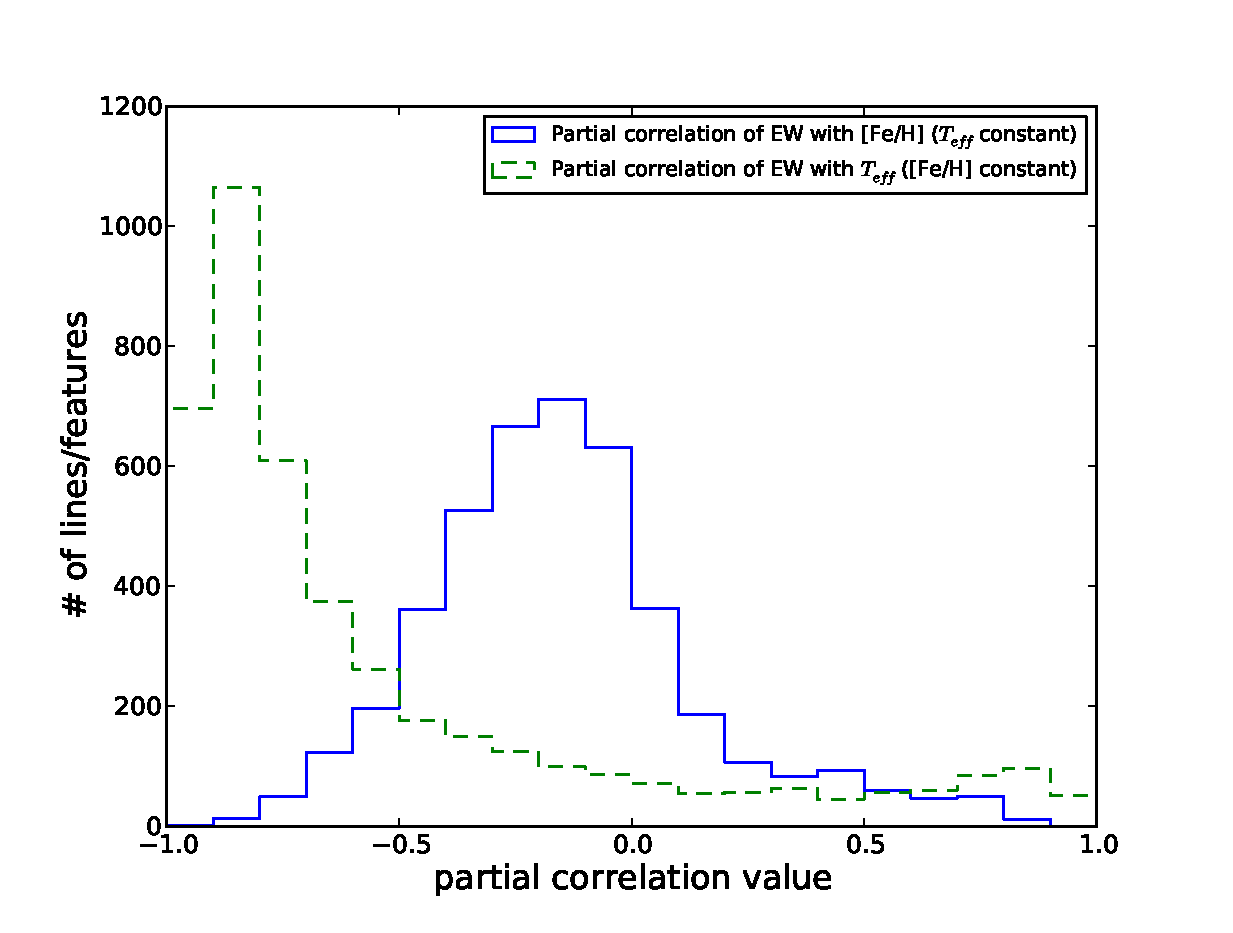
\includegraphics[scale=0.45]{../harpsm/all/pics_harpsmgtovpaper/pcorr.eps}
\end{center}
\caption{Histograms of the partial correlations of [Fe/H] (solid blue histogram) and $T_{eff}$ (dashed green histogram) }
\label{pcorr}
\end{figure}

Then we calculate a linear fit of the EWs with the metallicity (taken from \citet{Neves-2012}) and effective temperature (taken from \citet{Casagrande-2008}), using a least squares approach. For each EW $i$ and for each star $m$ we have,

\begin{equation}
W_{i,m} = \alpha_{i}[Fe/H]_{m}^{T} + \beta_{i}T_{eff m}^{T} + \gamma_{i}Ones_{m}^{T},
\label{first}
\end{equation}


where $W_{i,m}$ is a $i\times m$ matrix containing the EWs, and both $[Fe/H]_{m}$, and $T_{eff m}$ are $1\times m$ vectors. The $\alpha$ and the $\beta$ are the coefficients related to metallicity and effective temperature, respectively, while $\gamma$ is an independent coefficient. The Ones vector is a $1\times m$ vector of unit elements.

The error of each coefficient is calculated as

\begin{equation}
\epsilon_{i} = \sqrt{RSS.J_{i,i}},
\end{equation}
where RSS is the residual sum of squares, expressed as
\begin{equation}
RSS = \frac{\sum{(x-x_{i})^{2}}}{n_{obs}-n_{coef}},
\end{equation}
and $J$ is the estimate of the jacobian matrix around the solution. 

The total error of the coefficients can then be written as 

\begin{equation} 
\epsilon = \sqrt{\epsilon\alpha^{2}+\epsilon\beta^{2}+\epsilon\gamma^{2}}.
\end{equation}
Here we assume that both [Fe/H] and temperature are independent and do not correlate with each other. 

Our aim is to increase the metallicity precision using the photometric calibration as reference. In order to do this, we want to recover the values of the metallicity and temperature by doing a weighted least squares refit. To calculate the weights for the least squares refit we just invert the squared errors of the coefficients, and normalize the expression,

\begin{equation}
E_{i} = \frac{1/\epsilon_{i}^{2}}{\sum{1/\epsilon_{i}^{2}}}.
\label{weight}
\end{equation}

To invert the fit of Eq. \ref{first} we first take the calculated coefficients from the first fit and define the coefficient matrix as

\begin{equation}
C_{i,3} = \left[\begin{array}{ccc} \alpha_{1,1} & \beta_{1,2} & \gamma_{1,3} \\ \alpha_{2,1} & \beta_{2,2} & \gamma_{2,3} \\... & ... & ...\\ \alpha_{i,1} & \beta_{i,2} & \gamma_{i,3} \end{array}\right].
\end{equation}
Then we invert Eq. \ref{first}. After some operations we have 

\begin{equation}
[[Fe/H],Teff,Ind]_{3,m} = (C^{T}_{3,i}C_{i,3})^{-1}C^{T}_{3,i}W_{i,m},
\label{refit}
\end{equation}
where $C^{T}$ is the transpose of $C$ and $Ind$ is the value of the independent parameter. 

Finally, we use a \textit{levenberg-marquardt} algorithm and apply the weights (Eq. \ref{weight}) to Eq. \ref{refit}, recovering one value of metallicity and effective temperature for each star.

We also tried other methods, such as choosing groups of lines with a high correlation or partial correlation coefficients and then applying the same method as described in this subsection. However, the weighted least squares method using all 4441 lines performed best at minimizing both metallicity and effective temperature.

%\textcolor{red}{A plot of the best calibration here for Feh and teff?}

Using this method, we get a dispersion of metallicity and effective temperature of 0.08 dex and 70K respectively. \textbf{Figs. \ref{fehfeh} and \ref{teffteff} show the comparison between the values obtained in this work and the reference calibrations for metallicity and effective temperature, respectively}. We emphasize that we only get an improvement of the precision. The accuracy of the calibration, as well as systematic errors, are tied to the original determinations of both [Fe/H] and temperature.

\begin{figure}[h]
\begin{center}
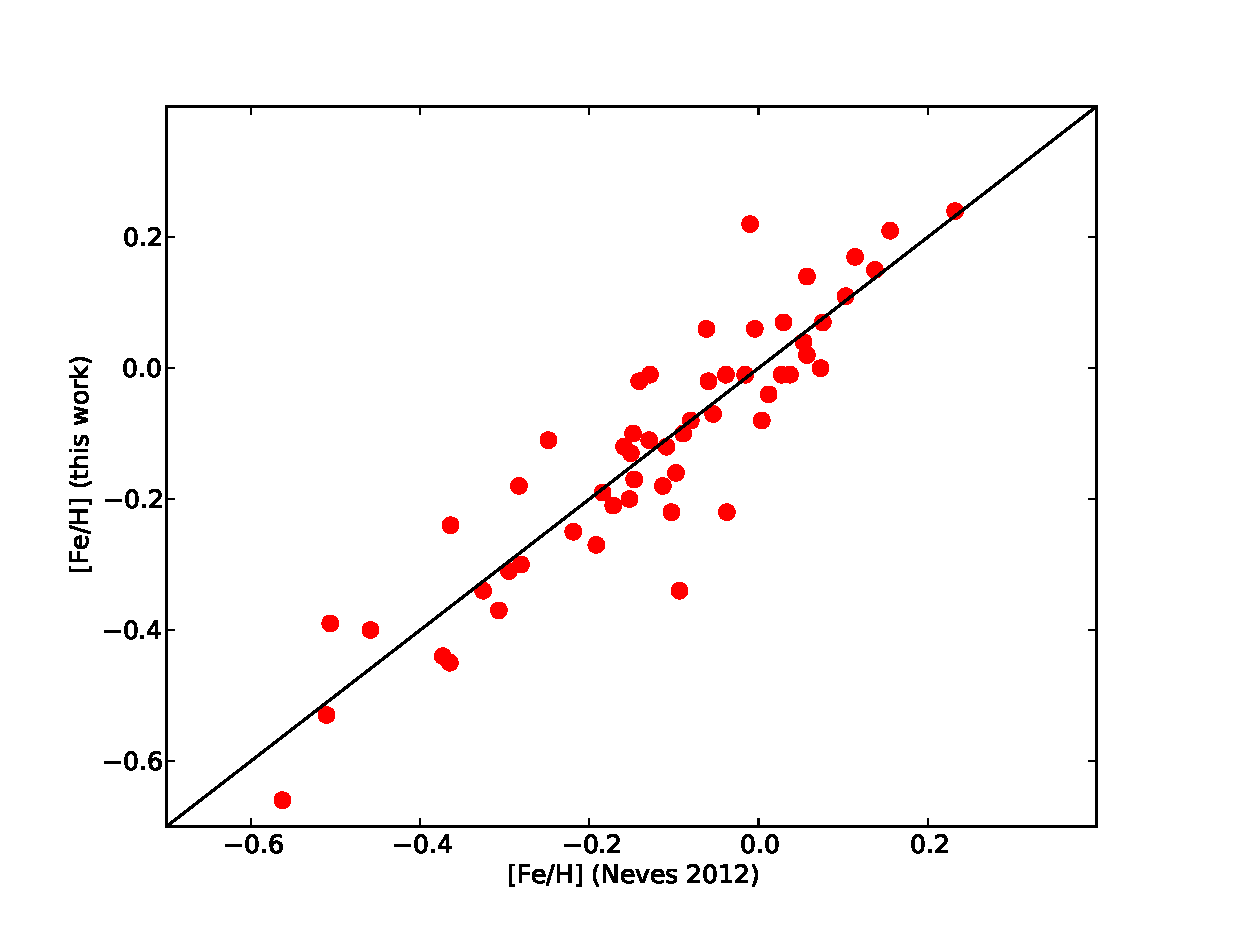
\includegraphics[scale=0.45]{../harpsm/all/pics_harpsmgtovpaper/fehfehn12.eps}
\end{center}
\caption{[Fe/H] comparison between this work and the photometric calibration of \citet{Neves-2012}.}
\label{fehfeh}
\end{figure}
%
%
\begin{figure}[h]
\begin{center}
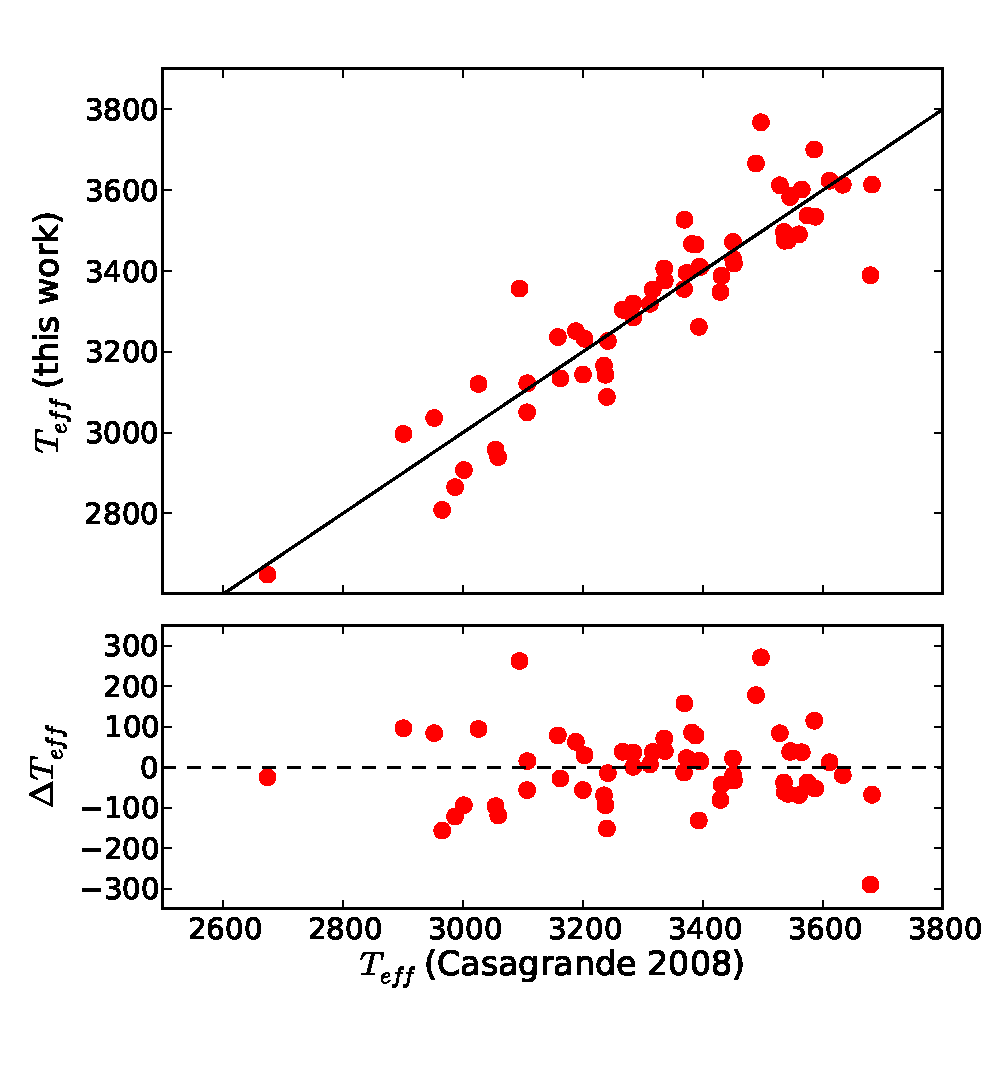
\includegraphics[scale=0.45]{../harpsm/all/pics_harpsmgtovpaper/teffteffc08.eps}
\end{center}
\caption{$T_{eff}$ comparison between this work and the photometric calibration of \citet{Casagrande-2008}.}
\label{teffteff}
\end{figure}

\onecolumn

%\begin{longtable}[b]
\begin{center}
\label{full_table} 
%\resizebox{9cm}{!}{
\begin{longtable}{ l r r r r r r r r r}
\caption{Sample} \\

%\toplabel{blabla}	
\hline
\hline
Star & $\alpha$ (2000) & $\delta$ (2000) & $\pi$ & $\pi$ src & Stype & V & $K_{S}$ & $M_{\star}$ & [Fe/H] \\
 &  & & [mas] & & & [mag] & [mag] & $[M_{\odot}]$ & [dex]\\
\hline
Gl1 & 00:05:25 & -37:21:23 & $230.4\pm 0.9$ & H & M3V &  8.6 & $4.501\pm0.030$ & $0.39\pm0.03$ & -0.23 \\
GJ1002 & 00:06:44 & -07:32:23 & $213.0\pm 3.6$ & H & M5.5V & 13.8 & $7.439\pm0.021$ & $0.11\pm0.01$ & -0.30 \\
Gl12 & 00:15:49 & +13:33:17 & $88.8\pm 3.5$ & H & M3 & 12.6 & $7.807\pm0.020$ & $0.22\pm0.02$ & -0.39 \\
LHS1134 & 00:43:26 & -41:17:36 & $101.0\pm16.0$ & R & M3 & 13.1 & $7.710\pm0.016$ & $0.20\pm0.01$ & -0.22 \\
Gl54.1 & 01:12:31 & -17:00:00 & $271.0\pm 8.4$ & H & M4.5V & 12.0 & $6.420\pm0.017$ & $0.13\pm0.01$ & -0.27 \\
L707-74 & 01:23:18 & -12:56:23 & $97.8\pm13.5$ & Y & m & 13.0 & $8.350\pm0.021$ & $0.15\pm0.02$ & -0.35 \\
Gl87 & 02:12:21 & +03:34:30 & $96.0\pm 1.7$ & H & M1.5 & 10.1 & $6.077\pm0.020$ & $0.45\pm0.03$ & -0.08 \\
Gl105B & 02:36:16 & +06:52:12 & $139.3\pm 0.5$ & H & M3.5V & 11.7 & $6.574\pm0.020$ & $0.25\pm0.02$ & -0.15 \\
CD-44-836A & 02:45:11 & -43:44:30 & $113.9\pm38.7$ & C & M4 & 12.3 & $7.270\pm0.024$ & $0.22\pm0.02$ & -0.24 \\
LHS1481 & 02:58:10 & -12:53:06 & $95.5\pm10.9$ & H & M2.5 & 12.7 & $8.199\pm0.026$ & $0.17\pm0.02$ & -0.73 \\
LP771-95A & 03:01:51 & -16:35:36 & $146.4\pm 2.9$ & H06 & M3 & 11.5 & $6.285\pm0.020$ & $0.24\pm0.02$ & -0.13 \\
LHS1513 & 03:11:36 & -38:47:17 & $130.0\pm20.0$ & R & M3.5 & 11.5 & $9.016\pm0.022$ & $0.09\pm0.02$ & -0.14 \\
GJ1057 & 03:13:23 & +04:46:30 & $117.1\pm 3.5$ & H & M5 & 13.9 & $7.833\pm0.024$ & $0.16\pm0.01$ & -0.01 \\
Gl145 & 03:32:56 & -44:42:06 & $93.1\pm 1.9$ & H & M2.5 & 11.5 & $6.907\pm0.016$ & $0.32\pm0.02$ & -0.27 \\
GJ1061 & 03:36:00 & -44:30:48 & $271.9\pm 1.3$ & H & M5.5V & 13.1 & $6.610\pm0.021$ & $0.12\pm0.01$ & -0.08 \\
GJ1065 & 03:50:44 & -06:05:42 & $105.4\pm 3.2$ & H & M4V & 12.8 & $7.751\pm0.020$ & $0.19\pm0.02$ & -0.08 \\
GJ1068 & 04:10:28 & -53:36:06 & $143.4\pm 1.9$ & H & M4.5 & 13.6 & $7.900\pm0.021$ & $0.13\pm0.01$ & -0.22 \\
Gl166C & 04:15:22 & -07:39:23 & $200.6\pm 0.2$ & H & M4.5V & 11.2 & $5.962\pm0.026$ & $0.23\pm0.02$ & -0.27 \\
Gl176 & 04:42:56 & +18:57:29 & $106.2\pm 2.5$ & H & M2.5 & 10.0 & $4.310\pm0.034$ & $0.50\pm0.03$ & 0.03 \\
LHS1723 & 05:01:57 & -06:56:47 & $187.9\pm 1.3$ & H & M3.5V & 12.2 & $6.736\pm0.024$ & $0.17\pm0.01$ & -0.29 \\
LHS1731 & 05:03:20 & -17:22:23 & $108.6\pm 2.7$ & H & M3.0V & 11.7 & $6.936\pm0.021$ & $0.27\pm0.02$ & -0.25 \\
Gl191 & 05:11:40 & -45:01:06 & $255.3\pm 0.9$ & H & M1 pV &  8.8 & $5.049\pm0.021$ & $0.27\pm0.03$ & -0.81 \\
Gl203 & 05:28:00 & +09:38:36 & $113.5\pm 5.0$ & H & M3.5V & 12.4 & $7.542\pm0.017$ & $0.19\pm0.02$ & -0.30 \\
Gl205 & 05:31:27 & -03:40:42 & $176.8\pm 1.2$ & H & M1.5V &  8.0 & $4.039\pm0.260$ & $0.60\pm0.07$ & 0.07 \\
Gl213 & 05:42:09 & +12:29:23 & $171.6\pm 4.0$ & H & M4V & 11.5 & $6.389\pm0.016$ & $0.22\pm0.02$ & -0.17 \\
Gl229 & 06:10:34 & -21:51:53 & $173.8\pm 1.0$ & H & M1V &  8.2 & $4.166\pm0.232$ & $0.58\pm0.06$ & -0.07 \\
HIP31293 & 06:33:43 & -75:37:47 & $110.9\pm 2.2$ & H & M3V & 10.5 & $5.862\pm0.024$ & $0.43\pm0.03$ & -0.02 \\
HIP31292 & 06:33:47 & -75:37:30 & $114.5\pm 3.2$ & H & M3/4V & 11.4 & $6.558\pm0.021$ & $0.31\pm0.02$ & -0.12 \\
G108-21 & 06:42:11 & +03:34:53 & $103.1\pm 8.5$ & H & M3.5 & 12.1 & $7.334\pm0.031$ & $0.23\pm0.02$ & -0.44 \\
Gl250B & 06:52:18 & -05:11:24 & $114.8\pm 0.4$ & H & M2.5V & 10.1 & $5.723\pm0.036$ & $0.45\pm0.03$ & -0.15 \\
Gl273 & 07:27:24 & +05:13:30 & $263.0\pm 1.4$ & H & M3.5V &  9.8 & $4.857\pm0.023$ & $0.29\pm0.02$ & -0.12 \\
LHS1935 & 07:38:41 & -21:13:30 & $94.3\pm 3.3$ & H & M3 & 11.7 & $7.063\pm0.023$ & $0.29\pm0.02$ & -0.36 \\
Gl285 & 07:44:40 & +03:33:06 & $167.9\pm 2.3$ & H & M4V & 11.2 & $5.698\pm0.017$ & $0.31\pm0.02$ & 0.24 \\
Gl299 & 08:11:57 & +08:46:23 & $146.3\pm 3.1$ & H & M4V & 12.8 & $7.660\pm0.026$ & $0.14\pm0.01$ & -0.51 \\
Gl300 & 08:12:41 & -21:33:12 & $125.8\pm 1.0$ & H & M3.5V & 12.1 & $6.705\pm0.027$ & $0.26\pm0.02$ & 0.05 \\
GJ2066 & 08:16:08 & +01:18:11 & $109.6\pm 1.5$ & H & M2 & 10.1 & $5.766\pm0.024$ & $0.46\pm0.03$ & -0.06 \\
GJ1123 & 09:17:05 & -77:49:17 & $110.9\pm 2.0$ & H & M4.5V & 13.1 & $7.448\pm0.021$ & $0.21\pm0.01$ & 0.13 \\
Gl341 & 09:21:38 & -60:16:53 & $95.6\pm 0.9$ & H & M0V &  9.5 & $5.587\pm0.021$ & $0.55\pm0.03$ & -0.04 \\
GJ1125 & 09:30:44 & +00:19:18 & $103.5\pm 3.9$ & H & M3.0V & 11.7 & $6.871\pm0.024$ & $0.29\pm0.02$ & -0.19 \\
Gl357 & 09:36:02 & -21:39:42 & $110.8\pm 1.9$ & H & M3V & 10.9 & $6.475\pm0.017$ & $0.33\pm0.03$ & -0.01 \\
Gl358 & 09:39:47 & -41:04:00 & $105.6\pm 1.6$ & H & M3.0V & 10.8 & $6.056\pm0.023$ & $0.42\pm0.03$ & 0.17 \\
Gl367 & 09:44:30 & -45:46:36 & $101.3\pm 3.2$ & H & M1 & 10.1 & $5.780\pm0.020$ & $0.49\pm0.03$ & -0.02 \\
GJ1129 & 09:44:48 & -18:12:48 & $90.9\pm 3.8$ & H & M3.5V & 12.5 & $7.257\pm0.020$ & $0.28\pm0.02$ & 0.06 \\
Gl382 & 10:12:17 & -03:44:47 & $127.1\pm 1.9$ & H & M2V &  9.3 & $5.015\pm0.020$ & $0.54\pm0.03$ & 0.08 \\
Gl388 & 10:19:36 & +19:52:12 & $204.6\pm 2.8$ & H & M4.5 &  9.4 & $4.593\pm0.017$ & $0.42\pm0.03$ & 0.06 \\
Gl393 & 10:28:55 & +00:50:23 & $141.5\pm 2.2$ & H & M2V &  9.7 & $5.311\pm0.023$ & $0.44\pm0.03$ & -0.08 \\
LHS288 & 10:44:32 & -61:11:35 & $209.7\pm 2.7$ & H & M5.5 & 13.9 & $7.728\pm0.027$ & $0.10\pm0.01$ & -0.48 \\
Gl402 & 10:50:52 & +06:48:30 & $147.9\pm 3.5$ & H & M4V & 11.7 & $6.371\pm0.016$ & $0.26\pm0.02$ & -0.21 \\
Gl406 & 10:56:29 & +07:00:54 & $419.1\pm 2.1$ & H & M6V & 13.4 & $6.084\pm0.017$ & $0.10\pm0.00$ & 0.15 \\
Gl413.1 & 11:09:31 & -24:36:00 & $93.0\pm 1.7$ & H & M2 & 10.4 & $6.097\pm0.023$ & $0.46\pm0.03$ & -0.10 \\
Gl433 & 11:35:27 & -32:32:23 & $112.6\pm 1.4$ & H & M2.0V &  9.8 & $5.623\pm0.021$ & $0.47\pm0.03$ & -0.21 \\
Gl438 & 11:43:20 & -51:50:23 & $119.0\pm10.2$ & R & M0 & 10.4 & $6.320\pm0.021$ & $0.33\pm0.03$ & -0.26 \\
Gl447 & 11:47:44 & +00:48:16 & $299.6\pm 2.2$ & H & M4 & 11.1 & $5.654\pm0.024$ & $0.17\pm0.01$ & -0.32 \\
Gl465 & 12:24:53 & -18:14:30 & $113.0\pm 2.5$ & H & M3V & 11.3 & $6.950\pm0.021$ & $0.26\pm0.02$ & -0.00 \\
Gl479 & 12:37:53 & -52:00:06 & $103.2\pm 2.3$ & H & M3V & 10.7 & $6.020\pm0.021$ & $0.43\pm0.03$ & 0.20 \\
LHS337 & 12:38:50 & -38:22:53 & $156.8\pm 2.0$ & H & M4.5V & 12.7 & $7.386\pm0.021$ & $0.15\pm0.01$ & -0.52 \\
Gl480.1 & 12:40:46 & -43:34:00 & $128.5\pm 3.9$ & H & M3.0V & 12.2 & $7.413\pm0.021$ & $0.18\pm0.02$ & -0.66 \\
Gl486 & 12:47:57 & +09:45:12 & $119.5\pm 2.7$ & H & M3.5 & 11.4 & $6.362\pm0.018$ & $0.32\pm0.02$ & 0.08 \\
Gl514 & 13:30:00 & +10:22:36 & $130.6\pm 1.1$ & H & M1V &  9.1 & $5.036\pm0.027$ & $0.53\pm0.03$ & -0.22 \\
Gl526 & 13:45:44 & +14:53:30 & $185.5\pm 1.1$ & H & M1.5V &  8.5 & $4.415\pm0.017$ & $0.50\pm0.03$ & 0.09 \\
Gl536 & 14:01:03 & -02:39:18 & $98.3\pm 1.6$ & H & M1 &  9.7 & $5.683\pm0.020$ & $0.52\pm0.03$ & 0.11 \\
Gl551 & 14:29:43 & -62:40:47 & $771.6\pm 2.6$ & H & M5.5 & 11.1 & $4.310\pm0.030$ & $0.12\pm0.01$ & 0.09 \\
Gl555 & 14:34:17 & -12:31:06 & $165.0\pm 3.3$ & H & M3.5V & 11.3 & $5.939\pm0.034$ & $0.28\pm0.02$ & 0.11 \\
Gl569A & 14:54:29 & +16:06:04 & $101.9\pm 1.7$ & H & M2.5 & 10.2 & $5.770\pm0.018$ & $0.49\pm0.03$ & -0.05 \\
Gl581 & 15:19:26 & -07:43:17 & $160.9\pm 2.6$ & H & M2.5V & 10.6 & $5.837\pm0.023$ & $0.30\pm0.02$ & -0.02 \\
Gl588 & 15:32:13 & -41:16:36 & $168.7\pm 1.3$ & H & M2.5V &  9.3 & $4.759\pm0.024$ & $0.47\pm0.03$ & -0.19 \\
Gl618A & 16:20:04 & -37:31:41 & $119.8\pm 2.5$ & H & M3V & 10.6 & $5.950\pm0.021$ & $0.39\pm0.03$ & -0.12 \\
Gl628 & 16:30:18 & -12:39:47 & $233.0\pm 1.6$ & H & M3V & 10.1 & $5.075\pm0.024$ & $0.30\pm0.02$ & -0.10 \\
Gl643 & 16:55:25 & -08:19:23 & $148.9\pm 4.0$ & H & M3.5V & 11.8 & $6.724\pm0.017$ & $0.21\pm0.02$ & -0.12 \\
Gl667C & 17:18:58 & -34:59:42 & $146.3\pm 9.0$ & H & M2V & 10.2 & $6.036\pm0.020$ & $0.30\pm0.03$ & -0.38 \\
Gl674 & 17:28:40 & -46:53:42 & $220.2\pm 1.4$ & H & M3V &  9.4 & $4.855\pm0.018$ & $0.35\pm0.03$ & -0.17 \\
Gl678.1A & 17:30:22 & +05:32:53 & $100.2\pm 1.1$ & H & M1V &  9.3 & $5.422\pm0.029$ & $0.57\pm0.03$ & -0.18 \\
Gl680 & 17:35:13 & -48:40:53 & $102.8\pm 2.8$ & H & M1.5 & 10.2 & $5.829\pm0.021$ & $0.47\pm0.03$ & 0.07 \\
Gl682 & 17:37:03 & -44:19:11 & $196.9\pm 2.1$ & H & M4.5V & 11.0 & $5.606\pm0.020$ & $0.27\pm0.02$ & 0.18 \\
Gl686 & 17:37:53 & +18:35:30 & $123.0\pm 1.6$ & H & M1 &  9.6 & $5.572\pm0.020$ & $0.45\pm0.03$ & -0.34 \\
Gl693 & 17:46:35 & -57:19:11 & $171.5\pm 2.3$ & H & M3.5V & 10.8 & $6.016\pm0.017$ & $0.26\pm0.02$ & -0.19 \\
Gl699 & 17:57:49 & +04:41:36 & $549.0\pm 1.6$ & H & M4V &  9.6 & $4.524\pm0.020$ & $0.16\pm0.01$ & -0.61 \\
Gl701 & 18:05:07 & -03:01:53 & $128.9\pm 1.4$ & H & M0V &  9.4 & $5.306\pm0.021$ & $0.48\pm0.03$ & -0.44 \\
GJ1224 & 18:07:33 & -15:57:47 & $132.6\pm 3.7$ & H & M4.5V & 13.6 & $7.827\pm0.027$ & $0.14\pm0.01$ & -0.26 \\
G141-29 & 18:42:44 & +13:54:17 & $93.3\pm11.5$ & H & M4 & 12.8 & $7.551\pm0.021$ & $0.23\pm0.02$ & -0.10 \\
Gl729 & 18:49:49 & -23:50:12 & $336.7\pm 2.0$ & H & M3.5V & 10.5 & $5.370\pm0.016$ & $0.17\pm0.01$ & -0.43 \\
GJ1232 & 19:09:51 & +17:40:07 & $93.6\pm 2.8$ & H & M4.5 & 13.6 & $7.902\pm0.020$ & $0.20\pm0.01$ & 0.21 \\
Gl752A & 19:16:55 & +05:10:05 & $170.4\pm 1.0$ & H & M3V &  9.1 & $4.673\pm0.020$ & $0.48\pm0.03$ & 0.06 \\
Gl754 & 19:20:48 & -45:33:30 & $169.2\pm 1.6$ & H & M4.5 & 12.2 & $6.845\pm0.026$ & $0.18\pm0.01$ & -0.08 \\
GJ1236 & 19:22:03 & +07:02:36 & $92.9\pm 2.5$ & H & M3 & 12.4 & $7.688\pm0.020$ & $0.22\pm0.02$ & -0.53 \\
GJ1256 & 20:40:34 & +15:29:57 & $102.0\pm 2.2$ & H & M4.5 & 13.4 & $7.749\pm0.031$ & $0.19\pm0.01$ & -0.01 \\
Gl803$^{\dag}$ & 20:45:10 & -31:20:30 & $100.9\pm 1.1$ & H & M0V e &  8.8 & $4.529\pm0.020$ & $0.75\pm0.03$ & 0.26 \\
LHS3583 & 20:46:37 & -81:43:12 & $77.1\pm21.2$ & C & M2.5 & 11.5 & $6.826\pm0.034$ & $0.40\pm0.03$ & -0.07 \\
LP816-60 & 20:52:33 & -16:58:30 & $175.0\pm 3.4$ & H & m & 11.4 & $6.199\pm0.021$ & $0.23\pm0.02$ & -0.17 \\
Gl832 & 21:33:34 & -49:00:36 & $201.9\pm 1.0$ & H & M1V &  8.7 & $4.473\pm0.050$ & $0.45\pm0.03$ & -0.35 \\
Gl846 & 22:02:10 & +01:24:00 & $97.6\pm 1.5$ & H & M0.5V &  9.2 & $5.322\pm0.023$ & $0.60\pm0.03$ & -0.00 \\
LHS3746 & 22:02:29 & -37:04:54 & $134.3\pm 1.3$ & H & M3.5 & 11.8 & $6.718\pm0.020$ & $0.24\pm0.02$ & -0.10 \\
Gl849 & 22:09:40 & -04:38:30 & $109.9\pm 2.1$ & H & M3V & 10.4 & $5.594\pm0.017$ & $0.49\pm0.03$ & 0.21 \\
GJ1265 & 22:13:42 & -17:41:12 & $96.0\pm 3.9$ & H & M4.5 & 13.6 & $8.115\pm0.018$ & $0.17\pm0.01$ & -0.29 \\
LHS3799 & 22:23:07 & -17:36:23 & $134.4\pm 4.9$ & H & M4.5V & 13.3 & $7.319\pm0.018$ & $0.18\pm0.01$ & 0.07 \\
Gl876 & 22:53:17 & -14:15:48 & $213.3\pm 2.1$ & H & M3.5V & 10.2 & $5.010\pm0.021$ & $0.34\pm0.02$ & 0.17 \\
Gl877 & 22:55:46 & -75:27:36 & $116.1\pm 1.2$ & H & M2.5 & 10.4 & $5.811\pm0.021$ & $0.43\pm0.03$ & 0.06 \\
Gl880 & 22:56:35 & +16:33:12 & $146.1\pm 1.0$ & H & M1.5V &  8.7 & $4.523\pm0.016$ & $0.58\pm0.03$ & 0.02 \\
Gl887 & 23:05:52 & -35:51:12 & $303.9\pm 0.9$ & H & M2V &  7.3 & $3.465\pm0.200$ & $0.47\pm0.05$ & -0.35 \\
LHS543 & 23:21:37 & +17:17:25 & $91.0\pm 2.9$ & H & M4 & 11.7 & $6.507\pm0.016$ & $0.40\pm0.02$ & 0.15 \\
Gl908 & 23:49:13 & +02:24:06 & $167.3\pm 1.2$ & H & M1V &  9.0 & $5.043\pm0.020$ & $0.42\pm0.03$ & -0.46 \\
LTT9759 & 23:53:50 & -75:37:53 & $100.1\pm 1.1$ & H & M... & 10.0 & $5.549\pm0.027$ & $0.54\pm0.03$ & 0.21 \\
\hline
\hline
\end{longtable}
\raggedright{
\small
$\pi$ src: (H) revised Hipparcos catalog \citep{van_Leeuwen-2007}; (R) \citep{Reid-1995}; (H06) \citep{Henry-2006}; (C) CNS4 catalog (Jahreiss, 
private comm.) \\
$^{\dag}$ Gl803 is a young ($\sim$20 Myr) M dwarf with a circumstellar disk \citep{Kalas-2004}. The equation to determine its mass may not be adequate for this age. \\}

\end{center}


\end{document}















%%%%%%%%%%%%%%%%%%%%%%%%%%%%%%%%%%%%%%%%%%%%%%%%%%%%%%%%%%%%%%
Examples for figures using graphicx
A guide "Using Imported Graphics in LaTeX2e"  (Keith Reckdahl)
is available on a lot of LaTeX public servers or ctan mirrors.
The file is : epslatex.pdf 
%%%%%%%%%%%%%%%%%%%%%%%%%%%%%%%%%%%%%%%%%%%%%%%%%%%%%%%%%%%%%%

%_____________________________________________________________
%                 A figure as large as the width of the column
%-------------------------------------------------------------
   \begin{figure}
   \centering
   \includegraphics[width=\textwidth]{empty.eps}
      \caption{Vibrational stability equation of state
               $S_{\mathrm{vib}}(\lg e, \lg \rho)$.
               $>0$ means vibrational stability.
              }
         \label{FigVibStab}
   \end{figure}
%
%_____________________________________________________________
%                                    One column rotated figure
%-------------------------------------------------------------
   \begin{figure}
   \centering
   \includegraphics[angle=-90,width=3cm]{empty.eps}
      \caption{Vibrational stability equation of state
               $S_{\mathrm{vib}}(\lg e, \lg \rho)$.
               $>0$ means vibrational stability.
              }
         \label{FigVibStab}
   \end{figure}
%
%_____________________________________________________________
%                        Figure with caption on the right side 
%-------------------------------------------------------------
   \begin{figure}
   \centering
   \includegraphics[width=3cm]{empty.eps}
      \caption{Vibrational stability equation of state
               $S_{\mathrm{vib}}(\lg e, \lg \rho)$.
               $>0$ means vibrational stability.
              }
         \label{FigVibStab}
   \end{figure}
%
%_____________________________________________________________
%
%_____________________________________________________________
%                                Figure with a new BoundingBox 
%-------------------------------------------------------------
   \begin{figure}
   \centering
   \includegraphics[bb=10 20 100 300,width=3cm,clip]{empty.eps}
      \caption{Vibrational stability equation of state
               $S_{\mathrm{vib}}(\lg e, \lg \rho)$.
               $>0$ means vibrational stability.
              }
         \label{FigVibStab}
   \end{figure}
%
%_____________________________________________________________
%
%_____________________________________________________________
%                                      The "resizebox" command 
%-------------------------------------------------------------
   \begin{figure}
   \resizebox{\textwidth}{!}
            {\includegraphics[bb=10 20 100 300,clip]{empty.eps}
      \caption{Vibrational stability equation of state
               $S_{\mathrm{vib}}(\lg e, \lg \rho)$.
               $>0$ means vibrational stability.
              }
         \label{FigVibStab}
   \end{figure}
%
%______________________________________________________________
%
%_____________________________________________________________
%                                             Simple A&A Table
%_____________________________________________________________
%
\begin{table}
\caption{Nonlinear Model Results}             % title of Table
\label{table:1}      % is used to refer this table in the text
\centering                          % used for centering table
\begin{tabular}{c c c c}        % centered columns (4 columns)
\hline\hline                 % inserts double horizontal lines
HJD & $E$ & Method\#2 & Method\#3 \\    % table heading 
\hline                        % inserts single horizontal line
   1 & 50 & $-837$ & 970 \\      % inserting body of the table
   2 & 47 & 877    & 230 \\
   3 & 31 & 25     & 415 \\
   4 & 35 & 144    & 2356 \\
   5 & 45 & 300    & 556 \\ 
\hline                                   %inserts single line
\end{tabular}
\end{table}
%
%_____________________________________________________________
%                                             Two column Table 
%_____________________________________________________________
%
\begin{table*}
\caption{Nonlinear Model Results}             
\label{table:1}      
\centering          
\begin{tabular}{c c c c l l l }     % 7 columns 
\hline\hline       
                      % To combine 4 columns into a single one 
HJD & $E$ & Method\#2 & \multicolumn{4}{c}{Method\#3}\\ 
\hline                    
   1 & 50 & $-837$ & 970 & 65 & 67 & 78\\  
   2 & 47 & 877    & 230 & 567& 55 & 78\\
   3 & 31 & 25     & 415 & 567& 55 & 78\\
   4 & 35 & 144    & 2356& 567& 55 & 78 \\
   5 & 45 & 300    & 556 & 567& 55 & 78\\
\hline                  
\end{tabular}
\end{table*}
%
%-------------------------------------------------------------
%                                          Table with notes 
%-------------------------------------------------------------
%
% A single note
\begin{table}[h]
\caption{\label{t7}Spectral types and photometry for stars in the
  region.}
\centering
\begin{tabular}{lccc}
\hline\hline
Star&Spectral type&RA(J2000)&Dec(J2000)\\
\hline
69           &B1\,V     &09 15 54.046 & $-$50 00 26.67\\
49           &B0.7\,V   &*09 15 54.570& $-$50 00 03.90\\
LS~1267~(86) &O8\,V     &09 15 52.787&11.07\\
24.6         &7.58      &1.37 &0.20\\
\hline
LS~1262      &B0\,V     &09 15 05.17&11.17\\
MO 2-119     &B0.5\,V   &09 15 33.7 &11.74\\
LS~1269      &O8.5\,V   &09 15 56.60&10.85\\
\hline
\end{tabular}
\tablefoot{ The top panel shows likely members of Pismis~11. The second
panel contains likely members of Alicante~5. The bottom panel
displays stars outside the clusters.}
\end{table}
%
% More notes
%
\begin{table}[h]
\caption{\label{t7}Spectral types and photometry for stars in the
  region.}
\centering
\begin{tabular}{lccc}
\hline\hline
Star&Spectral type&RA(J2000)&Dec(J2000)\\
\hline
69           &B1\,V     &09 15 54.046 & $-$50 00 26.67\\
49           &B0.7\,V   &*09 15 54.570& $-$50 00 03.90\\
LS~1267~(86) &O8\,V     &09 15 52.787&11.07\tablefootmark{a}\\
24.6         &7.58\tablefootmark{1}&1.37\tablefootmark{a}   &0.20\tablefootmark{a}\\
\hline
LS~1262      &B0\,V     &09 15 05.17&11.17\tablefootmark{b}\\
MO 2-119     &B0.5\,V   &09 15 33.7 &11.74\tablefootmark{c}\\
LS~1269      &O8.5\,V   &09 15 56.60&10.85\tablefootmark{d}\\
\hline
\end{tabular}
\tablefoot{ The top panel shows likely members of Pismis~11. The second
panel contains likely members of Alicante~5. The bottom panel
displays stars outside the clusters.\\
\tablefoottext{a}{Photometry for MF13, LS~1267 and HD~80077 from
Dupont et al.}
\tablefoottext{b}{Photometry for LS~1262, LS~1269 from
Durand et al.}
\tablefoottext{c}{Photometry for MO2-119 from
Mathieu et al.}
}
\end{table}
%
%-------------------------------------------------------------
%                                       Table with references 
%-------------------------------------------------------------
%
\begin{table*}[h]
 \caption[]{\label{nearbylistaa2}List of nearby SNe used in this work.}
\begin{tabular}{lccc}
 \hline \hline
  SN name &
  Epoch &
 Bands &
  References \\
 &
  (with respect to $B$ maximum) &
 &
 \\ \hline
1981B   & 0 & {\it UBV} & 1\\
1986G   &  $-$3, $-$1, 0, 1, 2 & {\it BV}  & 2\\
1989B   & $-$5, $-$1, 0, 3, 5 & {\it UBVRI}  & 3, 4\\
1990N   & 2, 7 & {\it UBVRI}  & 5\\
1991M   & 3 & {\it VRI}  & 6\\
\hline
\noalign{\smallskip}
\multicolumn{4}{c}{ SNe 91bg-like} \\
\noalign{\smallskip}
\hline
1991bg   & 1, 2 & {\it BVRI}  & 7\\
1999by   & $-$5, $-$4, $-$3, 3, 4, 5 & {\it UBVRI}  & 8\\
\hline
\noalign{\smallskip}
\multicolumn{4}{c}{ SNe 91T-like} \\
\noalign{\smallskip}
\hline
1991T   & $-$3, 0 & {\it UBVRI}  &  9, 10\\
2000cx  & $-$3, $-$2, 0, 1, 5 & {\it UBVRI}  & 11\\ %
\hline
\end{tabular}
\tablebib{(1)~\citet{branch83};
(2) \citet{phillips87}; (3) \citet{barbon90}; (4) \citet{wells94};
(5) \citet{mazzali93}; (6) \citet{gomez98}; (7) \citet{kirshner93};
(8) \citet{patat96}; (9) \citet{salvo01}; (10) \citet{branch03};
(11) \citet{jha99}.
}
\end{table}
%_____________________________________________________________
%                                 A rotated Table in landscape  
%  In the preamble, use:   \usepackage{lscape}
%-------------------------------------------------------------
\begin{landscape}
\begin{table*}
\caption{Summary for ISOCAM sources with mid-IR excess 
(YSO candidates).}\label{YSOtable}
\centering
\begin{tabular}{crrlcl} 
\hline\hline             
ISO-L1551 & $F_{6.7}$~[mJy] & $\alpha_{6.7-14.3}$ 
& YSO type$^{d}$ & Status & Comments\\
\hline
  \multicolumn{6}{c}{\it New YSO candidates}\\ % To combine 6 columns into a single one
\hline
  1 & 1.56 $\pm$ 0.47 & --    & Class II$^{c}$ & New & Mid\\
  2 & 0.79:           & 0.97: & Class II ?     & New & \\
  3 & 4.95 $\pm$ 0.68 & 3.18  & Class II / III & New & \\
  5 & 1.44 $\pm$ 0.33 & 1.88  & Class II       & New & \\
\hline
  \multicolumn{6}{c}{\it Previously known YSOs} \\
\hline
  61 & 0.89 $\pm$ 0.58 & 1.77 & Class I & \object{HH 30} & Circumstellar disk\\
  96 & 38.34 $\pm$ 0.71 & 37.5& Class II& MHO 5          & Spectral type\\
\hline
\end{tabular}
\end{table*}
\end{landscape}
%
%_____________________________________________________________
%                              Table longer than a single page  
%  In the preamble, use:              \usepackage{longtable}
%-------------------------------------------------------------
%          All long tables have to be placed at the end, after 
%                                        \end{thebibliography}
%
% In the text, at the place where the large table should appear
% add the command:
\addtocounter{table}{1}
% Tables counters will be well numbered.
%
\end{thebibliography}
% If table 2
\longtab{2}{
\begin{longtable}{lllrrr}
\caption{\label{kstars} Sample stars with absolute magnitude}\\
\hline\hline
Catalogue& $M_{V}$ & Spectral & Distance & Mode & Count Rate \\
\hline
\endfirsthead
\caption{continued.}\\
\hline\hline
Catalogue& $M_{V}$ & Spectral & Distance & Mode & Count Rate \\
\hline
\endhead
\hline
\endfoot
%%
Gl 33    & 6.37 & K2 V & 7.46 & S & 0.043170\\
Gl 66AB  & 6.26 & K2 V & 8.15 & S & 0.260478\\
Gl 68    & 5.87 & K1 V & 7.47 & P & 0.026610\\
         &      &      &      & H & 0.008686\\
Gl 86 
\footnote{Source not included in the HRI catalog. See Sect.~5.4.2 for details.}
         & 5.92 & K0 V & 10.91& S & 0.058230\\
\end{longtable}
}% End \longtab
%
%_____________________________________________________________
%                              Table longer than a single page
%                                             and in landscape 
%  In the preamble, use:       \usepackage{longtable,lscape}
%-------------------------------------------------------------
%          All long tables have to be placed at the end, after
%                                        \end{thebibliography}
%
% In the text, at the place where the large table should appear
% add the command:                        
\addtocounter{table}{1} 
% Tables counters will be well numbered.
%
\end{thebibliography}
% If table 2
\longtabL{2}{
\begin{landscape}
\begin{longtable}{lllrrr}
\caption{\label{kstars} Sample stars with absolute magnitude}\\
\hline\hline
Catalogue& $M_{V}$ & Spectral & Distance & Mode & Count Rate \\
\hline
\endfirsthead
\caption{continued.}\\
\hline\hline
Catalogue& $M_{V}$ & Spectral & Distance & Mode & Count Rate \\
\hline
\endhead
\hline
\endfoot
%%
Gl 33    & 6.37 & K2 V & 7.46 & S & 0.043170\\
Gl 66AB  & 6.26 & K2 V & 8.15 & S & 0.260478\\
Gl 68    & 5.87 & K1 V & 7.47 & P & 0.026610\\
         &      &      &      & H & 0.008686\\
Gl 86
\footnote{Source not included in the HRI catalog. See Sect.~5.4.2 for details.}
         & 5.92 & K0 V & 10.91& S & 0.058230\\
\end{longtable}
\end{landscape}
}% End \longtabL
%
% Online Material
%_____________________________________________________________
%        Online appendices have to be placed at the end, after
%                                        \end{thebibliography}
%-------------------------------------------------------------
\end{thebibliography}

\Online

\begin{appendix} %First online appendix
\section{Background galaxy number counts and shear noise-levels}
Because the optical images used in this analysis...

\begin{figure*}
\centering
\includegraphics[width=16.4cm,clip]{1787f24.ps}
\caption{Plotted above...}
\label{appfig}
\end{figure*}

Because the optical images...
\end{appendix}

\begin{appendix} %Second online appendix
These studies, however, have faced...
\end{appendix}

\end{document}
%
%_____________________________________________________________
%        Some tables or figures are in the printed version and
%                      some are only in the electronic version
%-------------------------------------------------------------
%
% Leave all the tables or figures in the text, at their right place 
% and use the commands \onlfig{}{} and \onltab{}{}. These elements
% will be automatically placed at the end, in the section
% Online material.

\documentclass{aa}
...
\begin{document}
text of the paper...
\begin{figure*}%f1
\includegraphics[width=10.9cm]{1787f01.eps}
\caption{Shown in greyscale is a...}
\label{cl12301}}
\end{figure*}
...
from the intrinsic ellipticity distribution.
% Figure 2 available electronically only
\onlfig{2}{
\begin{figure*}%f2
\includegraphics[width=11.6cm]{1787f02.eps}
\caption {Shown in greyscale...}
\label{cl1018}
\end{figure*}
}

% Figure 3 available electronically only
\onlfig{3}{
\begin{figure*}%f3
\includegraphics[width=11.2cm]{1787f03.eps}
\caption{Shown in panels...}
\label{cl1059}
\end{figure*}
}

\begin{figure*}%f4
\includegraphics[width=10.9cm]{1787f04.eps}
\caption{Shown in greyscale is...}
\label{cl1232}}
\end{figure*}

\begin{table}%t1
\caption{Complexes characterisation.}\label{starbursts}
\centering
\begin{tabular}{lccc}
\hline \hline
Complex & $F_{60}$ & 8.6 &  No. of  \\
...
\hline
\end{tabular}
\end{table}
The second method produces...

% Figure 5 available electronically only
\onlfig{5}{
\begin{figure*}%f5
\includegraphics[width=11.2cm]{1787f05.eps}
\caption{Shown in panels...}
\label{cl1238}}
\end{figure*}
}

As can be seen, in general the deeper...
% Table 2 available electronically only
\onltab{2}{
\begin{table*}%t2
\caption{List of the LMC stellar complexes...}\label{Properties}
\centering
\begin{tabular}{lccccccccc}
\hline  \hline
Stellar & RA & Dec & ...
...
\hline
\end{tabular}
\end{table*}
}

% Table 3 available electronically only
\onltab{3}{
\begin{table*}%t3
\caption{List of the derived...}\label{IrasFluxes}
\centering
\begin{tabular}{lcccccccccc}
\hline \hline
Stellar & $f12$ & $L12$ &...
...
\hline
\end{tabular}
\end{table*}
}
%
%-------------------------------------------------------------
%     For the online material, table longer than a single page
%                 In the preamble, use: \usepackage{longtable}
%       or for landscape option: \usepackage{longtable,lscape}
%-------------------------------------------------------------
\documentclass{aa}
\usepackage[varg]{txfonts}
\usepackage{graphicx}
\usepackage{longtable}

\begin{document}
text of the paper
% Table will be print automatically at the end, in the section Online material.
\onllongtab{3}{
\begin{longtable}{lrcrrrrrrrrl}
\caption{Line data and abundances ...}\\
\hline
\hline
Def & mol & Ion & $\lambda$ & $\chi$ & $\log gf$ & N & e &  rad & $\delta$ & $\delta$ 
red & References \\
\hline
\endfirsthead
\caption{Continued.} \\
\hline
Def & mol & Ion & $\lambda$ & $\chi$ & $\log gf$ & B & C &  rad & $\delta$ & $\delta$ 
red & References \\
\hline
\endhead
\hline
\endfoot
\hline
\endlastfoot
A & CH & 1 &3638 & 0.002 & $-$2.551 &  &  &  & $-$150 & 150 &  Jorgensen et al. (1996) \\                    
\end{longtable}
}% End onllongtab

% Or for landscape, large table:

\onllongtabL{3}{
\begin{landscape}
\begin{longtable}{lrcrrrrrrrrl}
...
\end{longtable}
\end{landscape}
}% End onllongtabL
